\documentclass{beamer} 

\usepackage{hayesmacros}
\usepackage{appendixnumberbeamer}
\usepackage{subcaption}

\usetheme{metropolis}
\setsansfont{Fira Sans}  % be sure to compile with XeLaTeX

\usepackage{natbib}
\usepackage{ulem}
\usepackage{fontawesome5}
\usepackage{twemojis}

\newtheorem{proposition}{Proposition}
\newtheorem{assumption}{Assumption}

\theoremstyle{remark}
\newtheorem*{remark}{Remark}

\setbeamercolor{background canvas}{bg=white}
\setbeamercolor{normal text}{fg=black}
\setbeamercolor{frametitle}{bg=black, fg=white}

\hypersetup{colorlinks,citecolor=cyan, urlcolor=cyan, linkcolor=black}

\title{Estimating network-mediated causal effects via spectral embeddings}
\date{2023-08-09 @ JSM 2023 \\ Recent Developments in Causal Inference}
\author{Alex Hayes, Mark Fredrickson \& Keith Levin}
\institute{Department of Statistics, University of Wisconsin-Madison}


\begin{document}

\maketitle

\begin{frame}{Causal mediation}

    \begin{columns}

        \column{0.5 \textwidth}

        \begin{table}[]
            \begin{tabular}{lcl}
                Treatment   & $T_i$          & $\in \set{0, 1} $     \\
                Outcome     & $Y_i$          & $\in \R$              \\
                Mediators   & $\X_{i \cdot}$ & $\in \R^{1 \times d}$ \\
                Confounders & $\C_{i \cdot}$ & $\in \R^{1 \times p}$
            \end{tabular}
        \end{table}

        \column{0.5 \textwidth}

        \begin{figure}[ht]
            \centering
            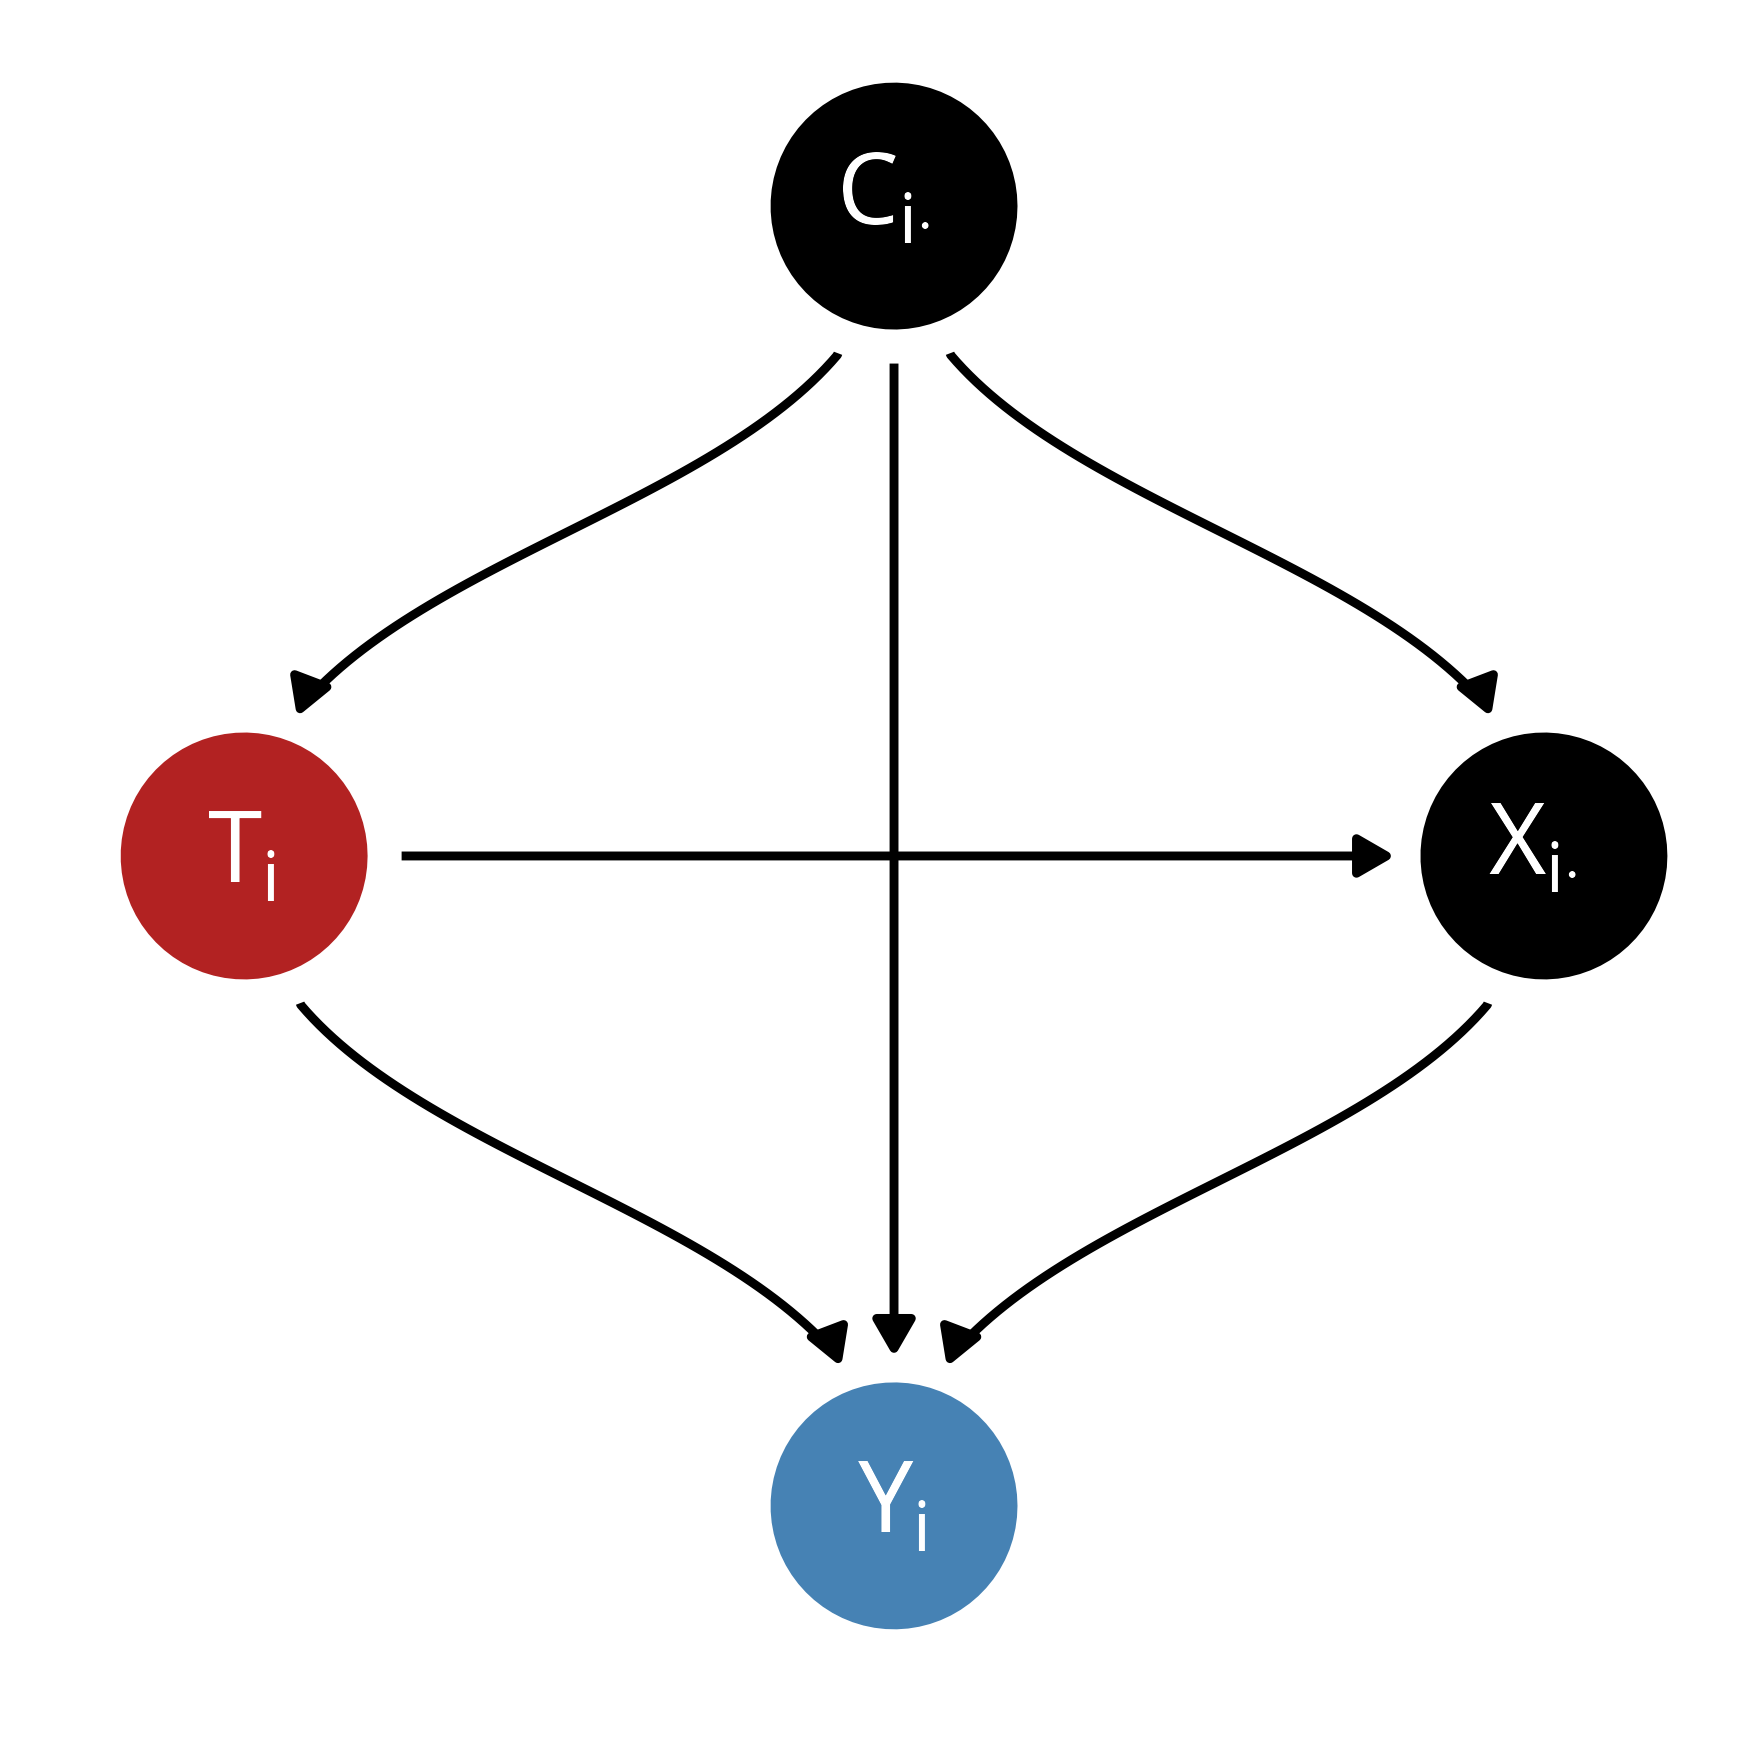
\includegraphics[width=0.9\textwidth]{figures/dags/mediating.png}
        \end{figure}
    \end{columns}

    Decompose effect of $T_i$ on $Y_i$:

    \begin{enumerate}
        \item Effect operating along $T_i \to Y_i$ path (direct)
        \item Effect operating along $T_i \to \X_{i \cdot} \to Y_i$ path (indirect)
    \end{enumerate}

\end{frame}

\begin{frame}{Decomposing the average treatment effect}

    $Y_i(t)$: counterfactual value of $Y_i$ when $T_i$ is set to $t$. The average treatment effect is
    \begin{align*}
        \ate = \E{Y_i(t) - Y_i(t^*)}
    \end{align*}
    which decomposes into the natural direct effect (not operating through $\X_{i \cdot}$) and natural indirect effect (operating through $\X_{i \cdot}$)
    \begin{align*}
        \ate & = \nde + \nie                                                    \\
        \nde & = \E{Y_i (t, \X_{i \cdot}(t^*)) - Y_i (t^*, \X_{i \cdot} (t^*))} \\
        \nie & = \E{Y_i (t, \X_{i \cdot}(t)) - Y_i (t, \X_{i \cdot} (t^*))}
    \end{align*}
\end{frame}

\section{This talk: social networks as mediators}

\begin{frame}{In particular: friends groups in social networks as mediators}

    \textbf{Motivating example:} friend groups mediate the effect of sex on smoking in an adolescent social network

    \begin{itemize}
        \item Girls smoke than boys
        \item Girls and boys in different friend groups
        \item Smoking varies with friend group
    \end{itemize}

\end{frame}

\begin{frame}{Teenage Friends and Lifestyle Study, Glasgow, 1996}
    \centering
    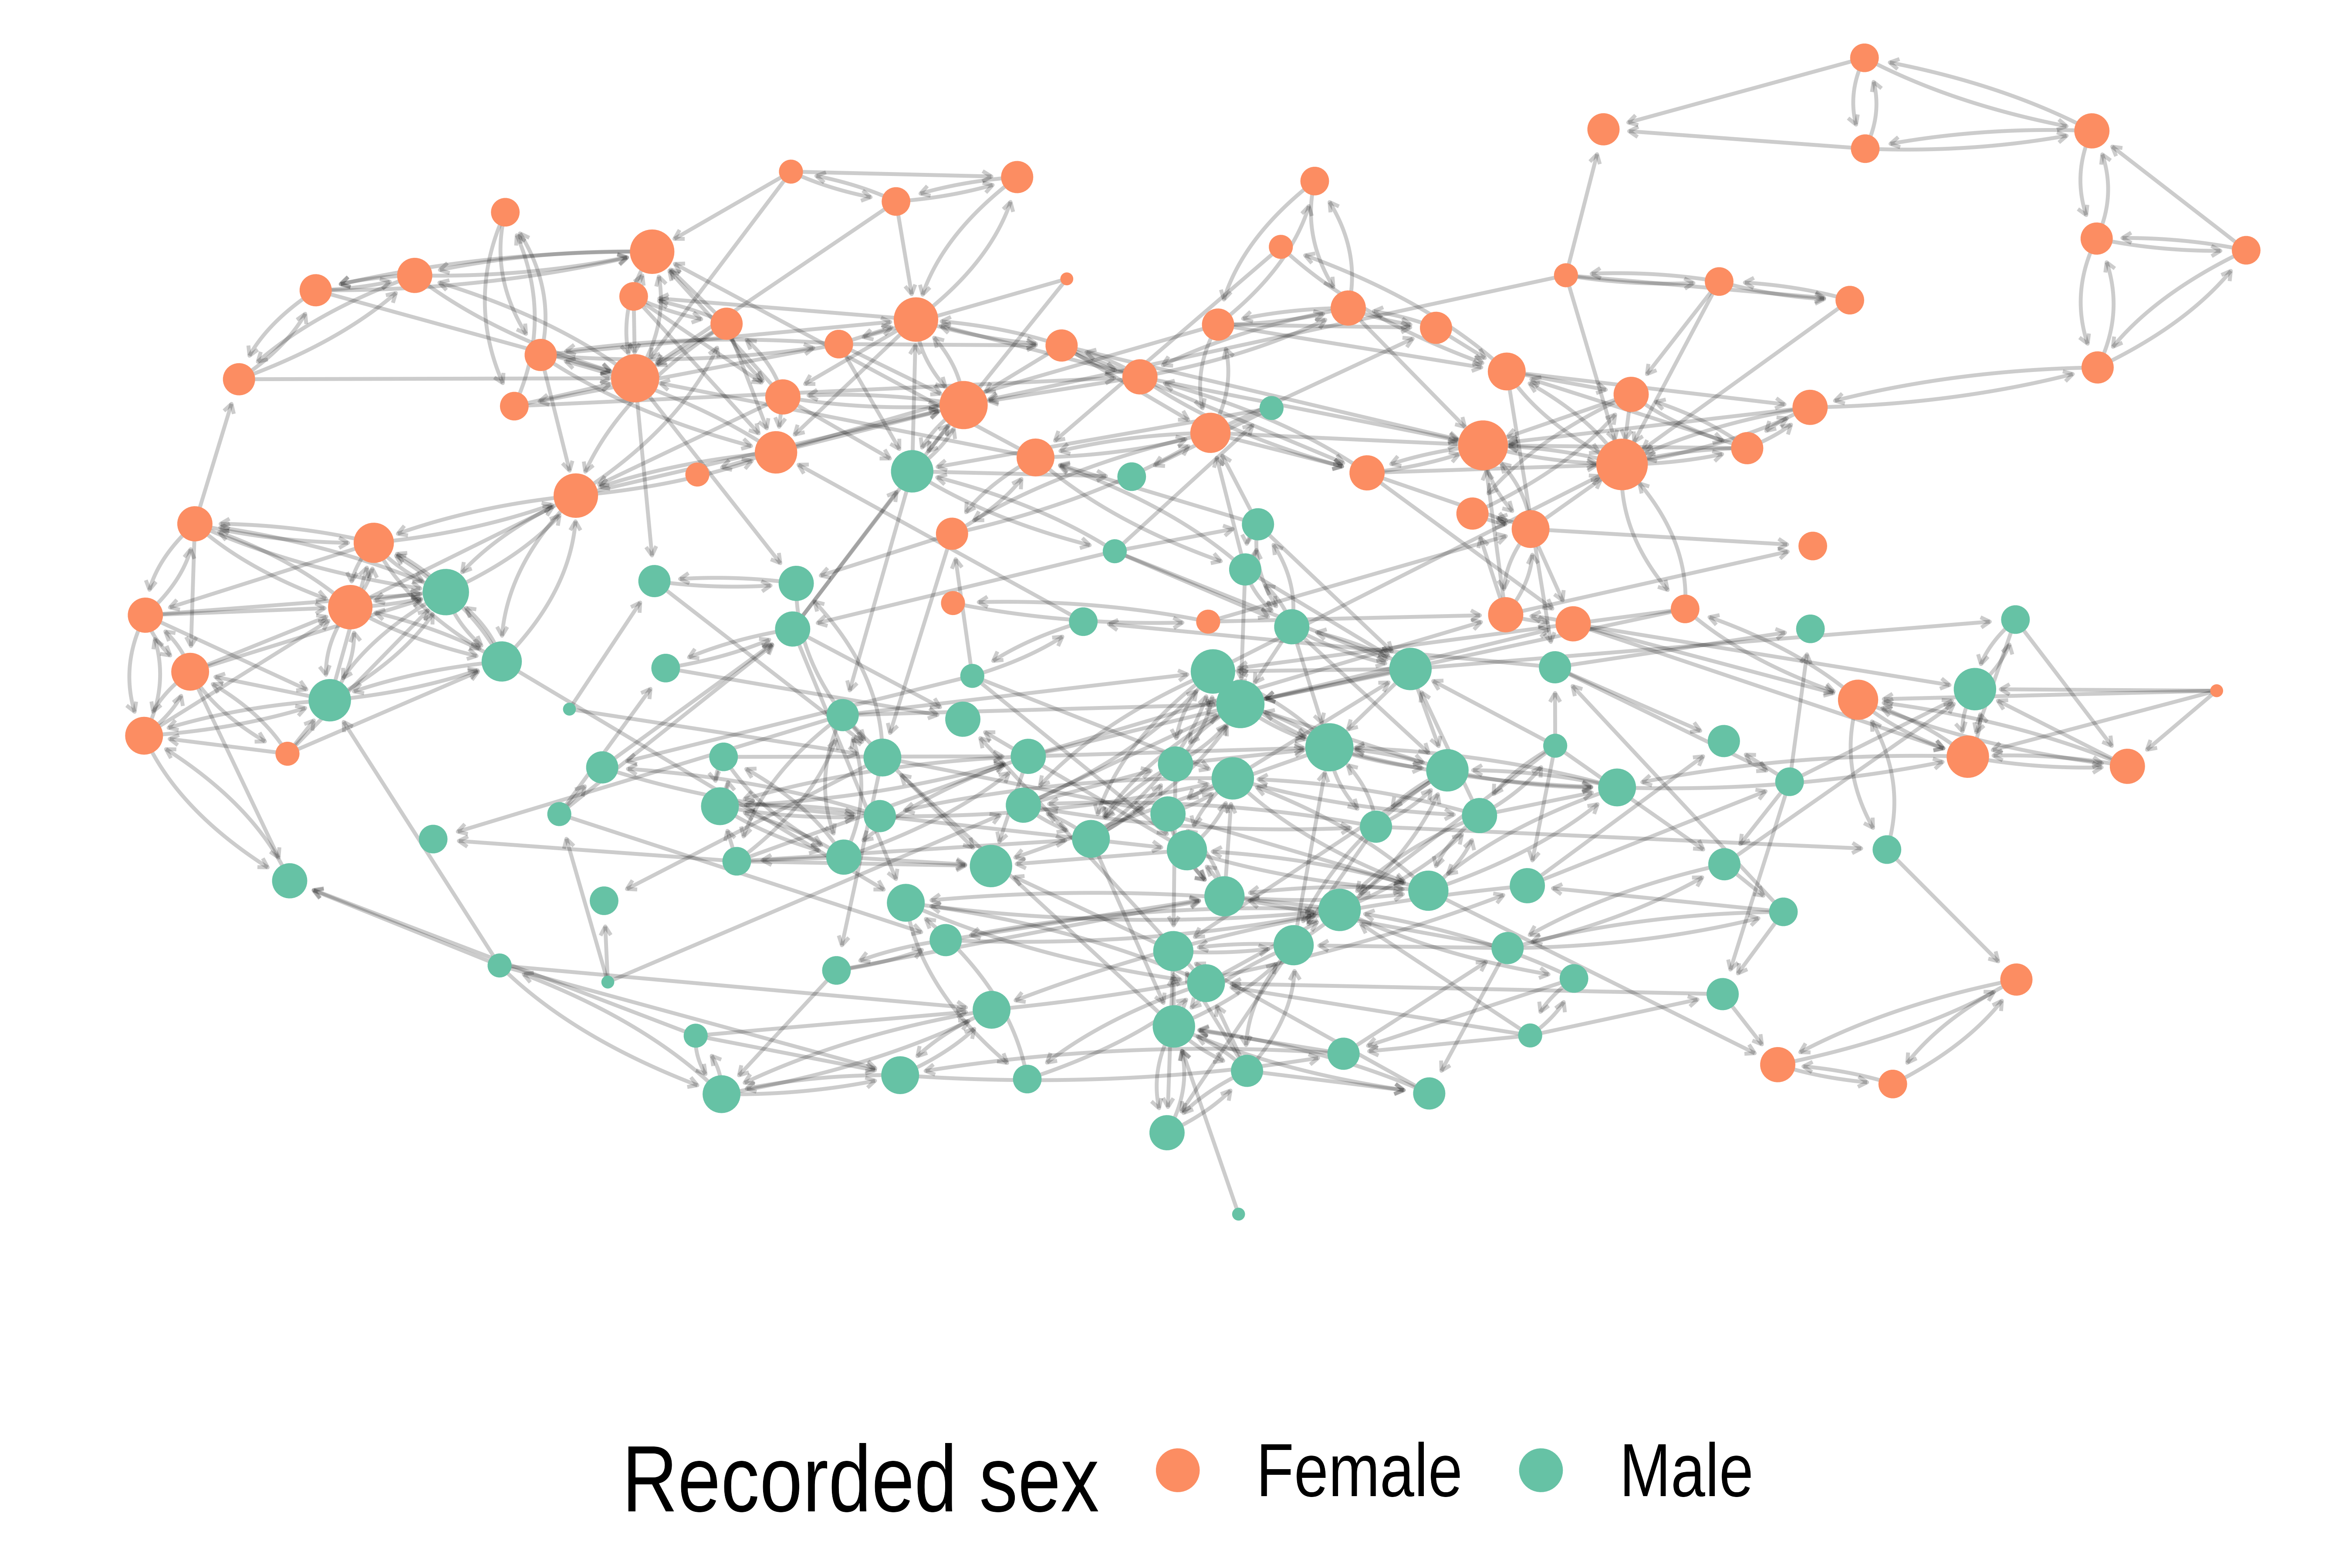
\includegraphics[width=\textwidth]{figures/glasgow/sex.png}
\end{frame}

\begin{frame}{Teenage Friends and Lifestyle Study, Glasgow, 1996}
    \centering
    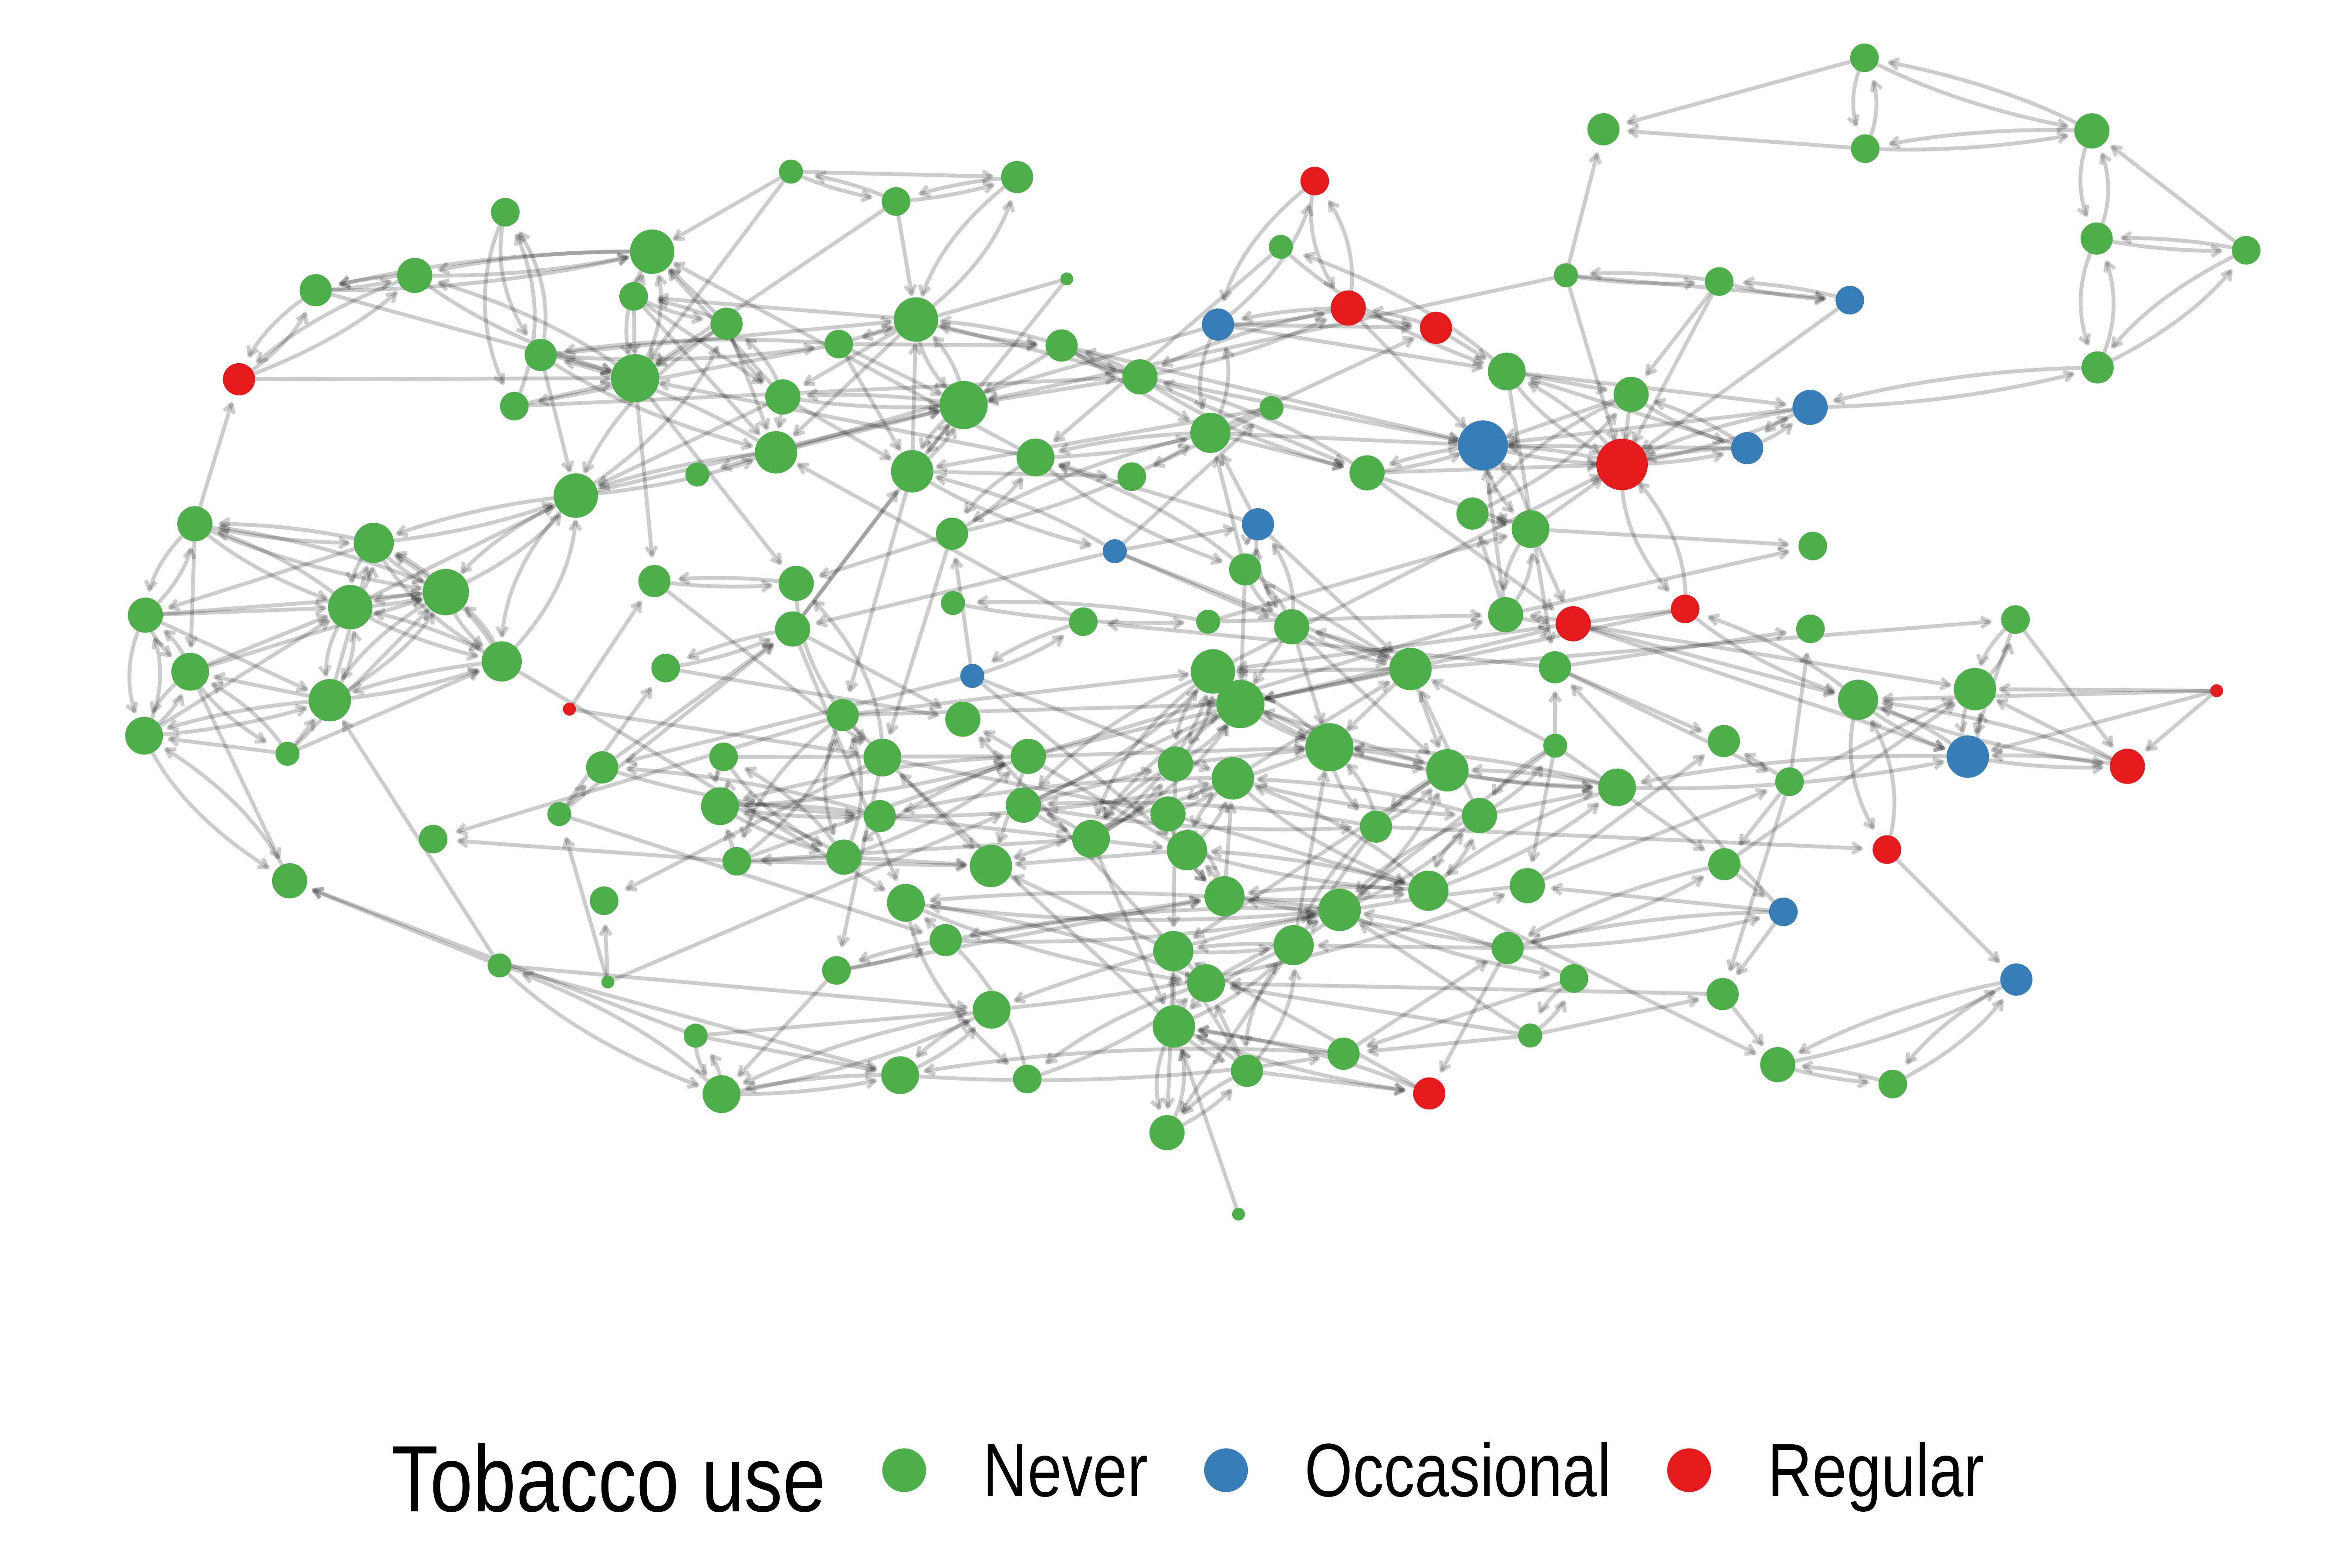
\includegraphics[width=\textwidth]{figures/glasgow/tobacco.png}
\end{frame}

\begin{frame}{Mediation on a social network}

    \begin{figure}[ht]
        \centering
        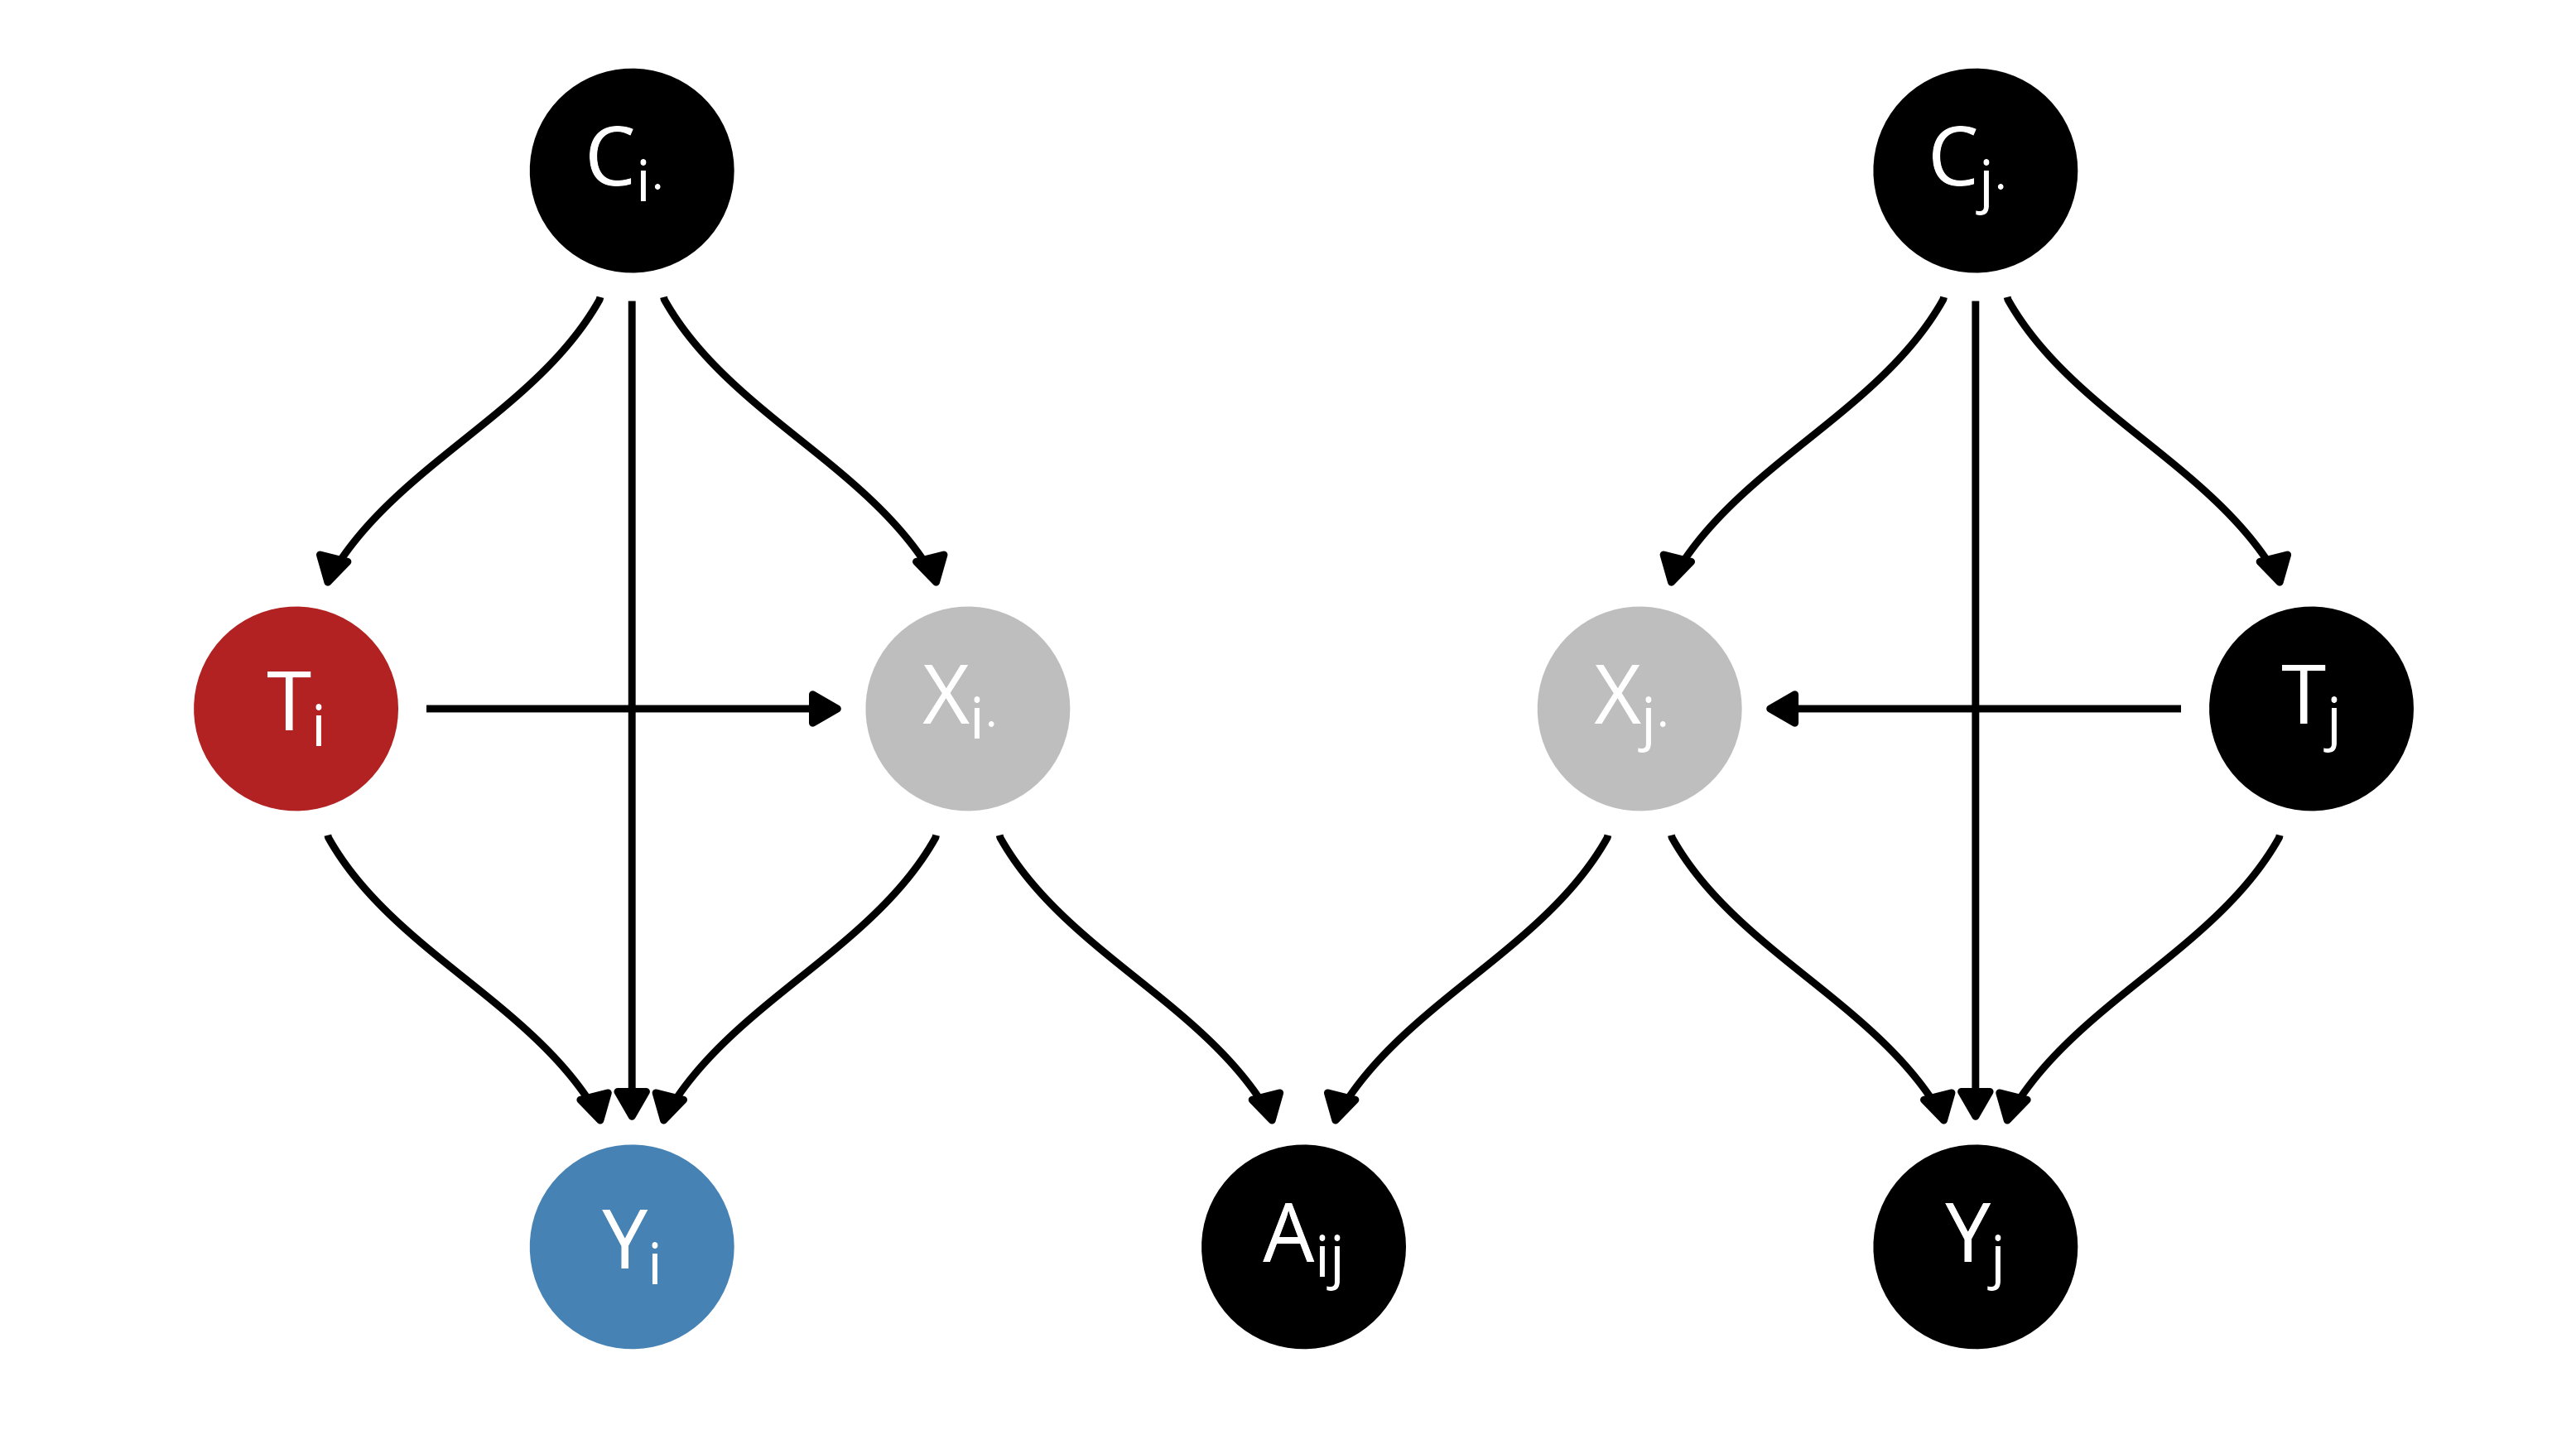
\includegraphics[width=0.8\textwidth]{figures/dags/homophily-mediating.png}
        \label{fig:mediating}
    \end{figure}

    \scriptsize

    \begin{table}[]
        \begin{tabular}{lcl}
            Adjacency matrix & $A$            & $\in \R^{n \times n}$ \\
            Edge $i \sim j$  & $A_{ij}$       & $\in \R$              \\
            Treatment        & $T_i$          & $\in \set{0, 1}$      \\
            Outcome          & $Y_i$          & $\in \R$              \\
            Confounders      & $\C_{i \cdot}$ & $\in \R^{1 \times p}$ \\
            Friend group     & $\X_{i \cdot}$ & $\in \R^{1 \times d}$
        \end{tabular}
    \end{table}
\end{frame}

\begin{frame}{The challenge: the friend groups $\X_{i \cdot}$ are not observed!}

    Solution: estimate friend groups $\X_{i \cdot}$ using community models!

    We use a semi-parametric estimator that accommodates:

    \begin{itemize}
        \item Stochastic blockmodels
        \item Degree-corrected stochastic blockmodels
        \item Mixed-membership stochastic blockmodels
        \item Overlapping stochastic blockmodels
        \item Random dot product graphs
        \item Etc
    \end{itemize}

\end{frame}

\begin{frame}{Intuition: stochastic blockmodels}

    \begin{columns}
        \column{0.45\textwidth}

        \begin{figure}
            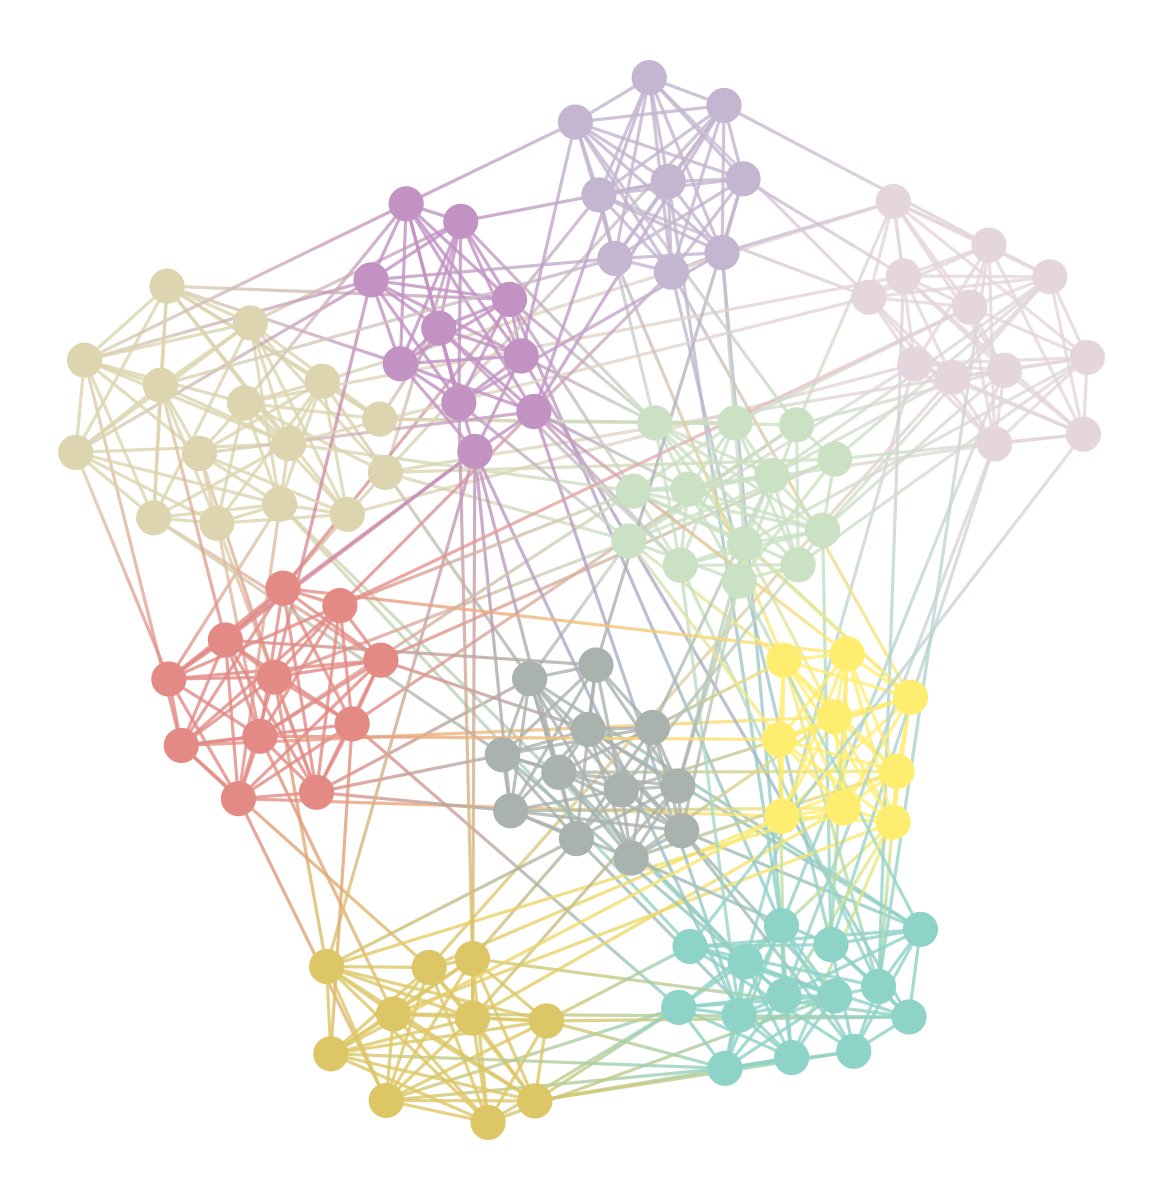
\includegraphics[width=\textwidth]{figures/assortative.png}
        \end{figure}

        \column{0.55\textwidth}

        $d$ ``blocks'' or communities

        $\X_{i \cdot} \in \set{0, 1}^d$ one-hot indicator of node $i$'s block

        \vspace{4mm}

        $\X$ is latent (i.e. unobserved)

        \vspace{4mm}

        $B \in [0, 1]^{d \times d}$ inter-block edge probabilities

        \vspace{4mm}

        Friendships depend on group memberships and $B$

        $\P[\X]{A_{ij} = 1} = \X_{i \cdot} B \X_{j \cdot}^T$

    \end{columns}

\end{frame}

\begin{frame}{Returning to the structural causal model for a moment}

    \centering

    \begin{figure}
        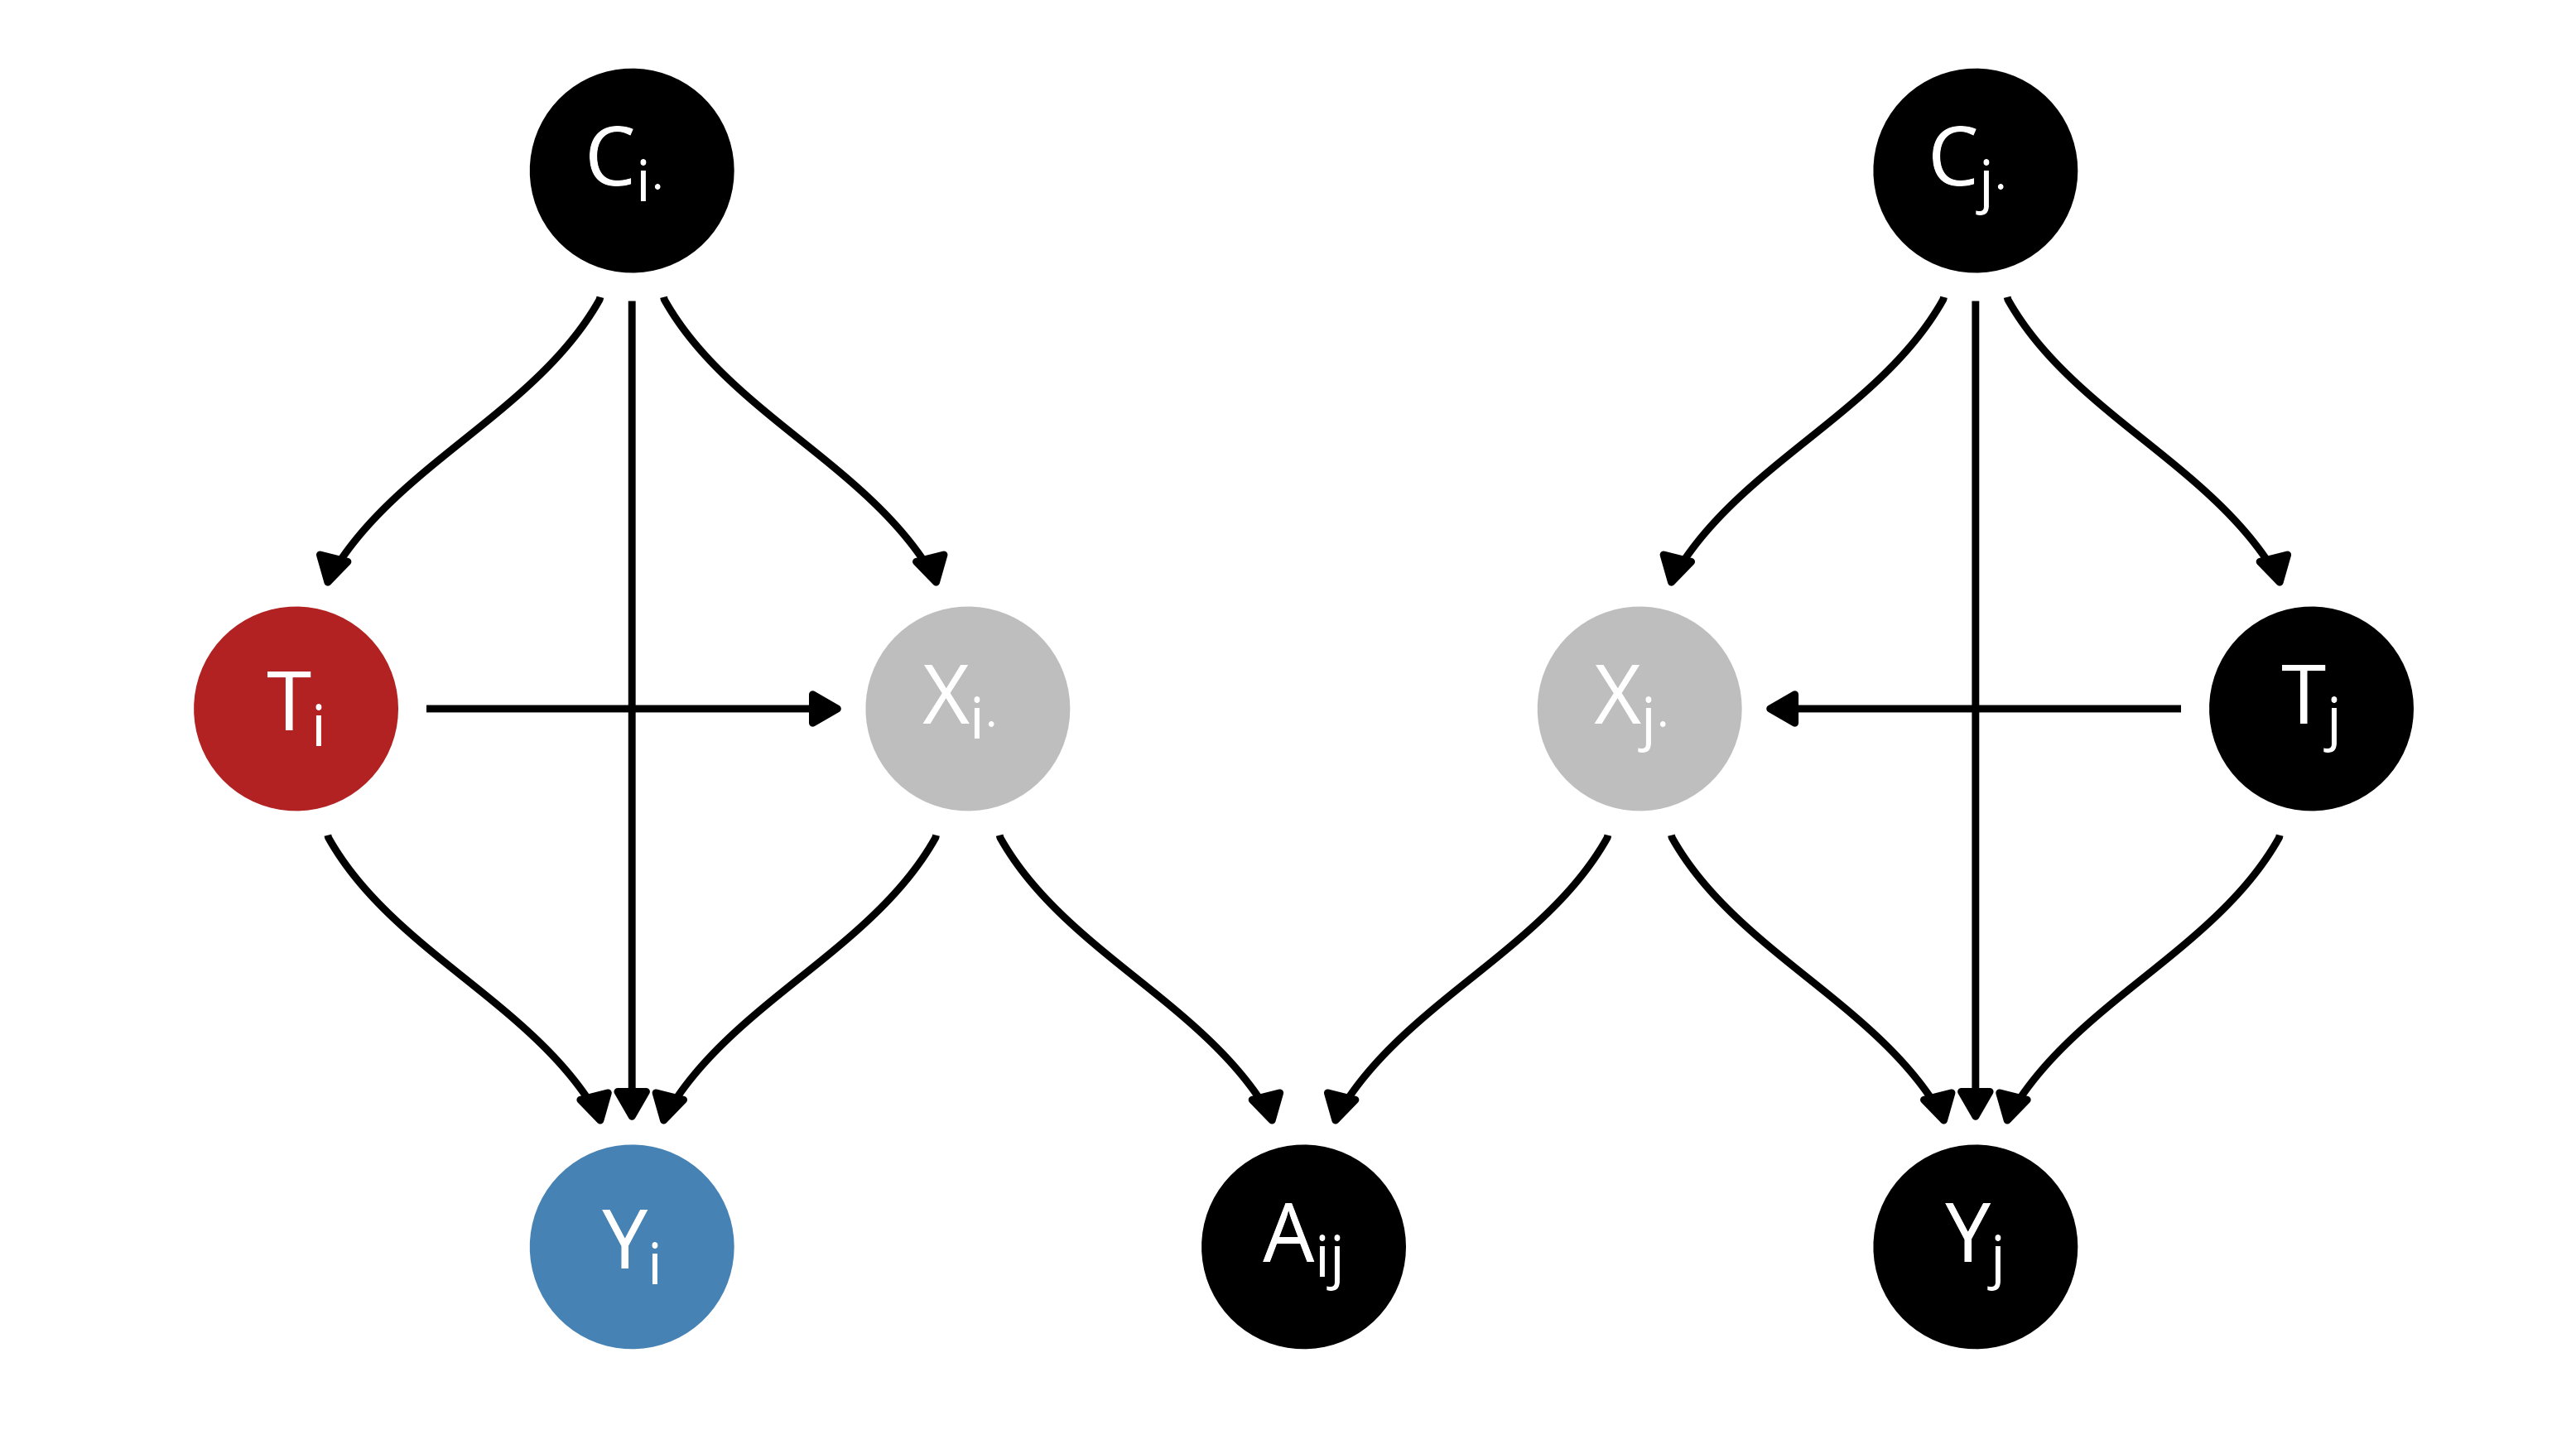
\includegraphics[scale=0.7]{figures/dags/homophily-mediating.png}
    \end{figure}

\end{frame}

\begin{frame}{Mediation estimators require $\X$, which is unknown}

    We will estimate $X$ and plug our estimate into standard estimators!

    \begin{definition}[ASE]

        Given a network $A$, the $\widehat{d}$-dimensional \emph{adjacency spectral embedding} of $A$ is

        \begin{align*}
            \Xhat = \Uhat \Shat^{1/2}
        \end{align*}

        \noindent where $\Uhat \Shat \Uhat^T$ is the rank-$\widehat{d}$ truncated singular value decomposition of $A$.

    \end{definition}

    \textbf{Note that the analyst must specify $\widehat{d}$}

\end{frame}

% \begin{frame}{Uniform consistency of the adjacency spectral embedding}

%     Well-known that $\Xhat$ is a good estimate of $\X$

%     \begin{lemma}

%         Under a suitably well-behaved network model, if $\widehat{d}$ is correctly specified or consistently estimated, there is some $d \times d$ orthogonal matrix $Q$ such that
%         \begin{equation*}
%             \max_{i \in [n]} \, \norm*{\Xhat_{i \cdot} - \X_{i \cdot} Q} = \op{1}.
%         \end{equation*}

%     \end{lemma}

% \end{frame}


\begin{frame}{Semi-parametric regression estimators}

    Under the assumption that:
    \begin{equation*}
        \begin{aligned}
            \underbrace{\E[T_i, \C_{i \cdot}, \X_{i \cdot}]{Y_i}}_{\R}
             & = \underbrace{\betazero}_{\R}
            + \underbrace{T_i}_{\{0, 1\}} \underbrace{\betat}_{\R}
            + \underbrace{\C_{i \cdot}}_{\R^{1 \times p}} \underbrace{\betac}_{\R^{p}}
            + \underbrace{\X_{i \cdot}}_{\R^{1 \times d}} \underbrace{\betax}_{\R^d}, \\
            \underbrace{\E[T_i, \C_{i \cdot}]{\X_{i \cdot}}}_{\R^{1 \times d}}
             & = \underbrace{\thetazero}_{\R^{1 \times d}}
            + \underbrace{T_i}_{\{0, 1\}} \underbrace{\thetat}_{\R^{1 \times d}}
            + \underbrace{\C_{i \cdot}}_{\R^{1 \times p}} \underbrace{\Thetac}_{\R^{p \times d}}
            + \underbrace{T_i}_{\{0, 1\}} \underbrace{\C_{i \cdot}}_{\R^{1 \times p}} \underbrace{\Thetatc}_{\R^{p \times d}}.
        \end{aligned}
    \end{equation*}
    Then:
    \begin{align*}
        \ndef & = \paren*{t - t^*} \, \betat                                                        \\
        \nief & = \paren*{t - t^*} \, \thetat \, \betax + (t - t^*) \, \mu_c \, \Thetatc \, \betax.
    \end{align*}

\end{frame}

\begin{frame}{A regression model for friend group membership}

    \centering

    \begin{figure}
        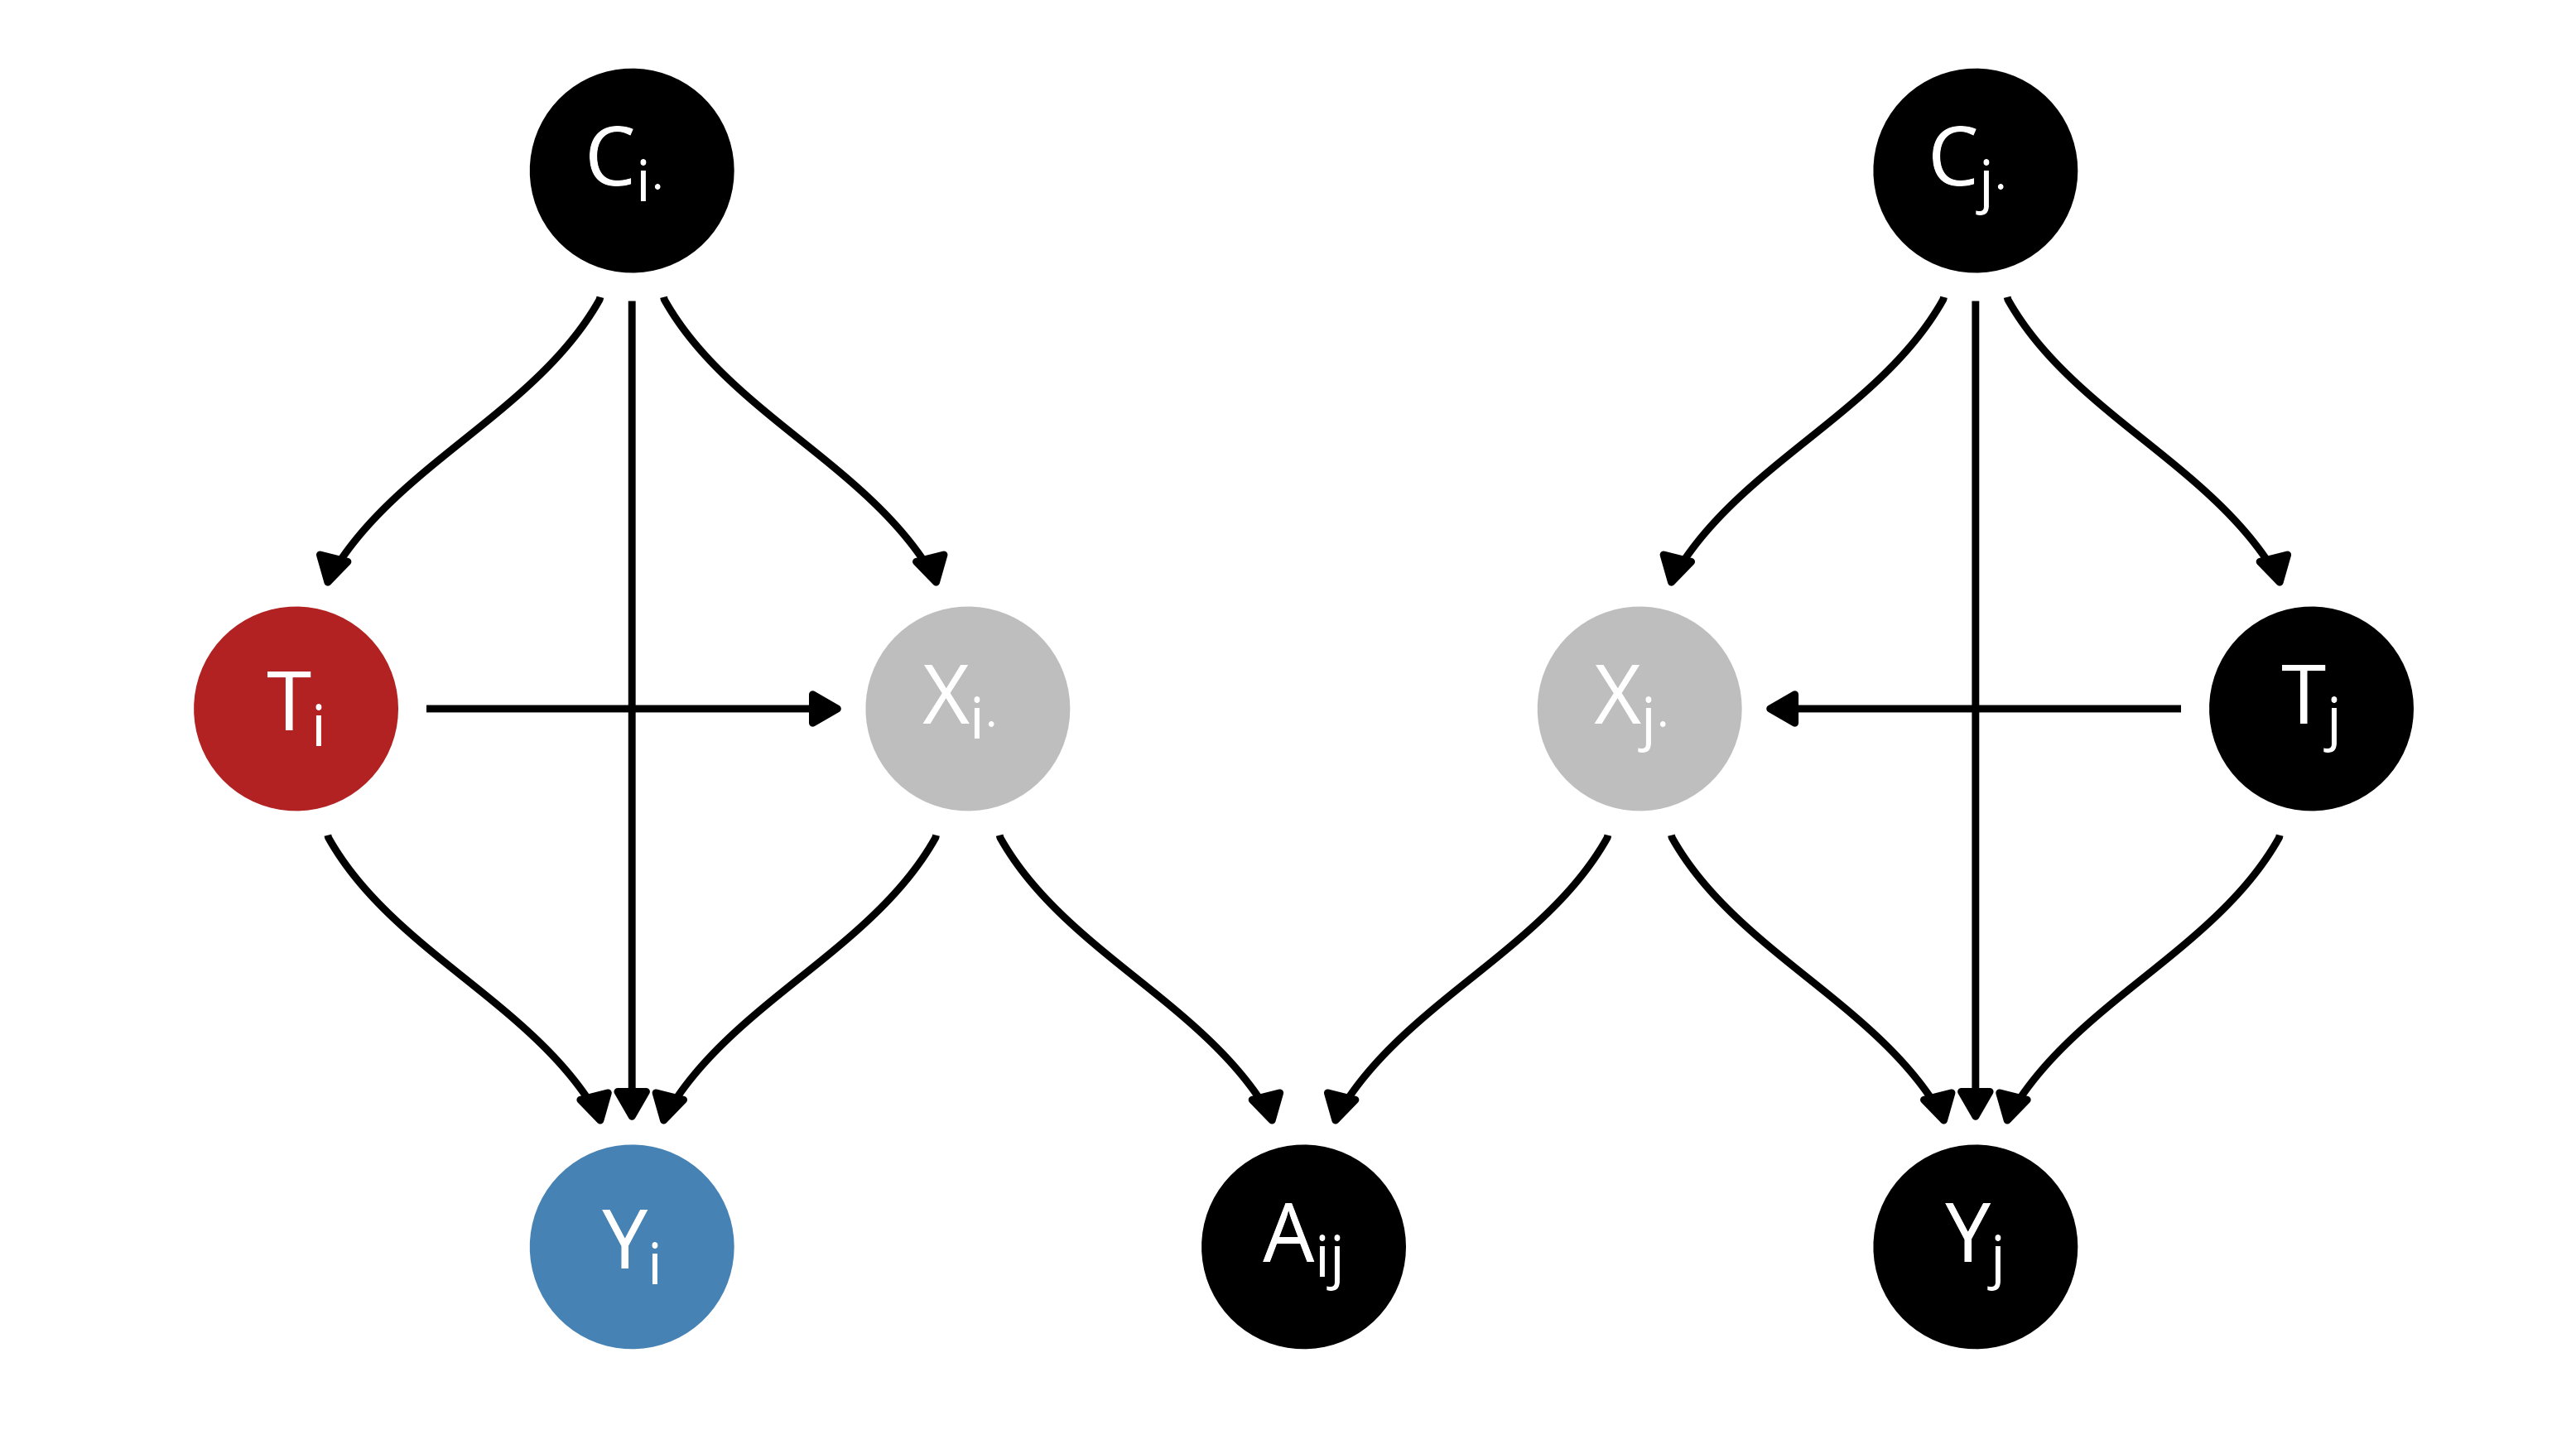
\includegraphics[scale=0.5]{figures/dags/homophily-mediating.png}
    \end{figure}
    Idea: interventions $T_i$ can cause community membership $\X_{i \cdot}$
    \begin{align*}
        \underbrace{\E[T_i, \C_{i \cdot}]{\X_{i \cdot}}}_{\R^{1 \times d}}
         & = \underbrace{\thetazero}_{\R^{1 \times d}}
        + \underbrace{T_i}_{\{0, 1\}} \underbrace{\thetat}_{\R^{1 \times d}}
        + \underbrace{\C_{i \cdot}}_{\R^{1 \times p}} \underbrace{\Thetac}_{\R^{p \times d}}
        + \underbrace{T_i}_{\{0, 1\}} \underbrace{\C_{i \cdot}}_{\R^{1 \times p}} \underbrace{\Thetatc}_{\R^{p \times d}}.
    \end{align*}

\end{frame}

\begin{frame}{A regression model for outcomes}

    \centering

    \begin{figure}
        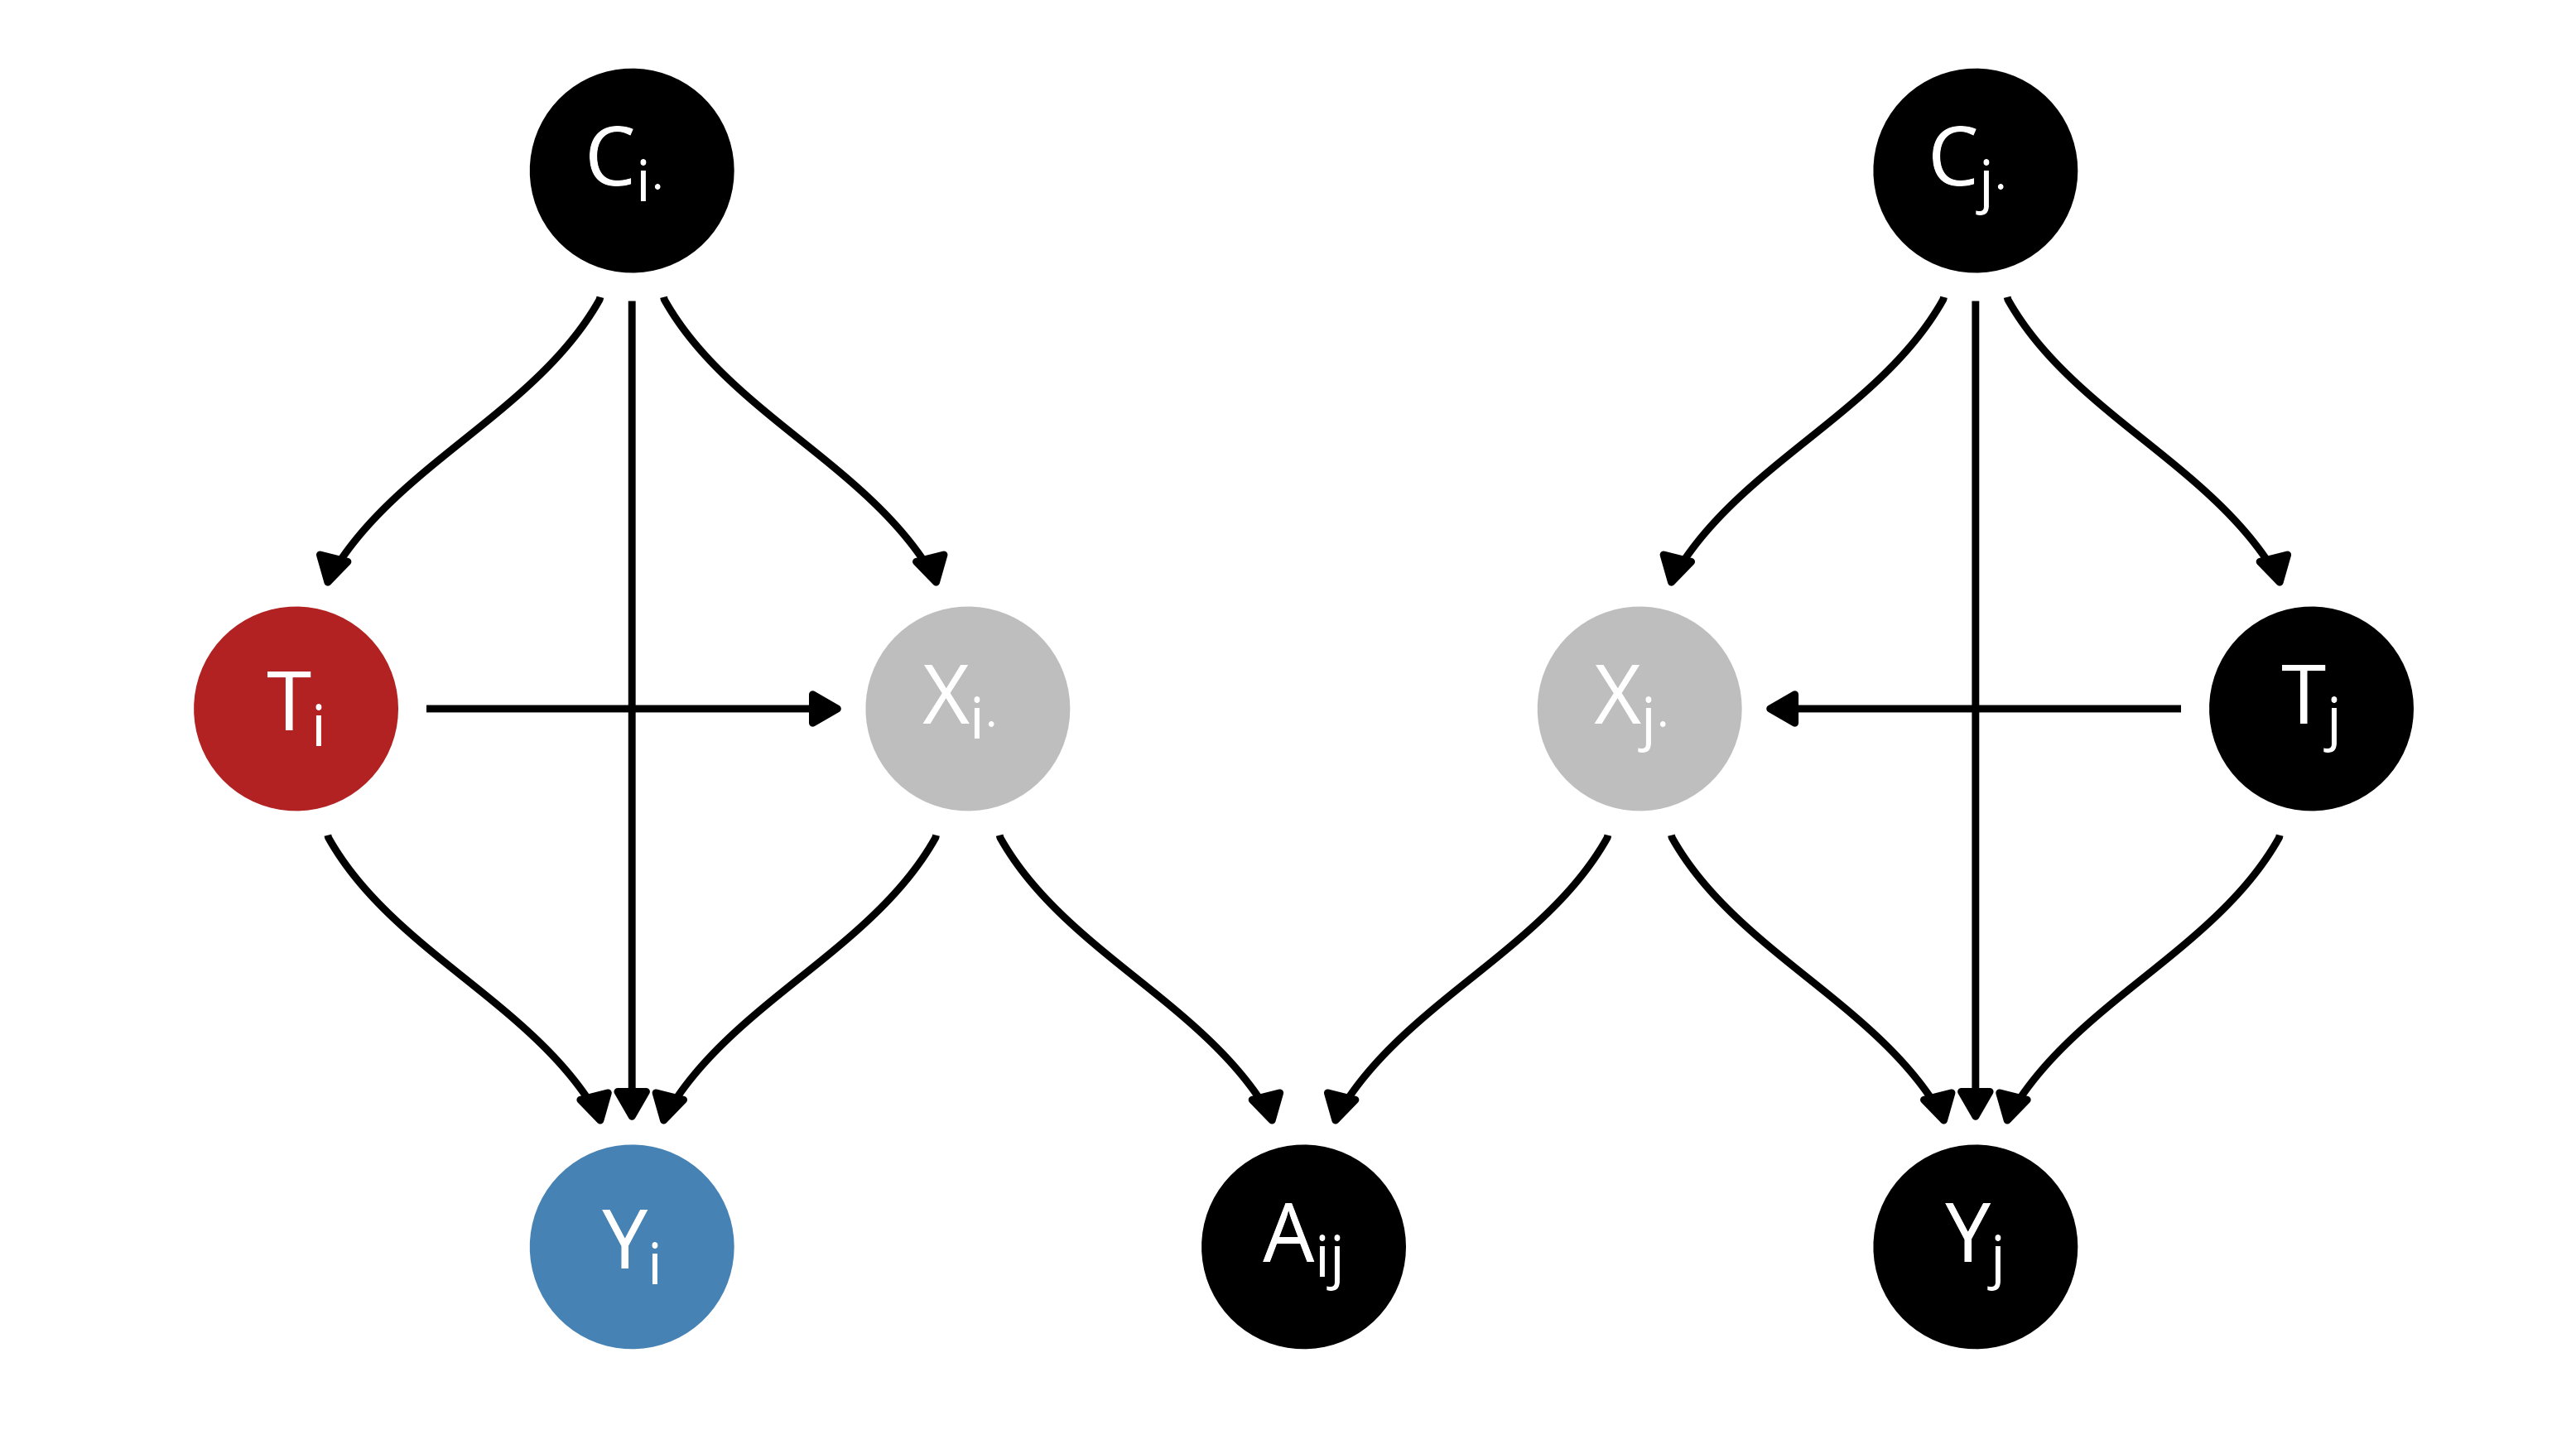
\includegraphics[scale=0.5]{figures/dags/homophily-mediating.png}
    \end{figure}

    Idea: community membership $\X_{i \cdot}$ can cause outcomes $Y_i$
    \begin{align*}
        \underbrace{\E[T_i, \C_{i \cdot}, \X_{i \cdot}]{Y_i}}_{\R}
         & = \underbrace{\betazero}_{\R}
        + \underbrace{T_i}_{\{0, 1\}} \underbrace{\betat}_{\R}
        + \underbrace{\C_{i \cdot}}_{\R^{1 \times p}} \underbrace{\betac}_{\R^{p}}
        + \underbrace{\X_{i \cdot}}_{\R^{1 \times d}} \underbrace{\betax}_{\R^d}
    \end{align*}

\end{frame}

\begin{frame}{$\Xhat$ can be plugged in for $\X$ just fine}

    Let $\Dhat = \begin{bmatrix} 1 & T & \C  & \Xhat \end{bmatrix} \in \R^{n \times (2 + p + d)}$ and $\Wfull = \begin{bmatrix} 1 & T & \C  & T \cdot \C \end{bmatrix} \in \R^{n \times (2 p + 2)}$.

    We estimate $\betaw$ and $\betax$ via ordinary least squares as follows
    \begin{equation*}
        \begin{bmatrix}
            \betazerohat \\
            \betathat    \\
            \betachat    \\
            \betaxhat
        \end{bmatrix}
        = \paren*{\Dhat^T \Dhat}^{-1} \Dhat^T Y.
    \end{equation*}
    Similarly, we estimate $\Theta$ via ordinary least squares as
    \begin{equation*}
        \Thetahat
        = \paren*{\Wfull^T \Wfull}^{-1} \Wfull^T \Xhat.
    \end{equation*}
\end{frame}

\begin{frame}{Causal estimators}

    To estimate $\nde$ and $\nie$ in our semi-parametric setting, we combine regression coefficients from the network regression models:
    \begin{align*}
        \cdehat & = \ndehat = \paren*{t - t^*} \, \betathat                                                                              & \text{and} \\
        \niehat & = \paren*{t - t^*} \, \thetathat \, \betaxhat + \paren*{t - t^*} \cdot \widehat{\mu}_c \cdot \Thetatchat \, \betaxhat.
    \end{align*}
    It's standard to fit two regressions and multiply coefficients to estimate an indirect effect like this \citep{vanderweele_mediation_2014}.

\end{frame}

\begin{frame}{Main result}

    \begin{theorem}[Regression coefficients are asymptotically normal]

        \vspace{2mm}

        Under some mild assumptions, there is an unknown orthogonal matrix $Q$ such that
        \begin{equation*}
            \begin{aligned}
                \sqrt{ n } \,
                 & \Sigmahatbeta^{-1/2}
                \begin{pmatrix}
                    \betawhat - \betaw \\
                    Q \, \betaxhat - \betax
                \end{pmatrix}
                \to
                \Normal{0}{I_d}, and     \\
                \sqrt{ n } \,
                 & \Sigmahattheta^{-1/2}
                \begin{pmatrix}
                    \vecc \paren*{\Thetahat \, Q^T} - \Thetavec
                \end{pmatrix}
                \to
                \Normal{0}{I_{p d}}.
            \end{aligned}
        \end{equation*}
        \noindent where $\Sigmahattheta^{-1/2}$ and $\Sigmahatbeta^{-1/2}$ are the typical heteroscedasticity robust covariance estimators, with $\Xhat$ plugged in for $\X$.
    \end{theorem}
\end{frame}

\begin{frame}{Corollary}

    \begin{theorem}[Causal estimators are asymptotically normal]

        \vspace{2mm}

        Under the same statistical assumptions as before, plus mediating homophily,
        \begin{align*}
            \sqrt{n \, \sigmahatnde} \paren*{\ndehat - \nde}
             & \to
            \Normal{0}{1}, \text { and } \\
            \sqrt{n \, \sigmahatnie} \paren*{\niehat - \nie}
             & \to
            \Normal{0}{1}.
        \end{align*}
        \noindent where $\sigmahatnde$ and $\sigmahatnie$ are rather unfriendly variance estimators derived via the delta method and the previous theorem.

    \end{theorem}

\end{frame}

% \section{Data example (if there is time)}

% \begin{frame}{Glasgow data}

%     TODO

% \end{frame}


\begin{frame}{Thank you! Questions?}

    Read the manuscript at \url{https://arxiv.org/abs/2212.12041}

    R package \href{https://github.com/alexpghayes/netmediate}{netmediate}

    \textbf{Stay in touch}

    \begin{itemize}
        \item[] \faIcon{twitter} \href{https://twitter.com/alexpghayes}{@alexpghayes}
        \item[] \faIcon[regular]{envelope} \href{mailto:alex.hayes@wisc.edu}{alex.hayes@wisc.edu}
        \item[] \faIcon{wordpress} \url{https://www.alexpghayes.com} % \faIcon{sitemap} \faIcon{firefox-browser} 
        \item[] \faIcon{github} \url{https://github.com/alexpghayes}
    \end{itemize}

    \textbf{I'm looking for a post-doc, say hi if this work interests you!}
\end{frame}

\appendix

\begin{frame}{Disambiguation: contagion ($Y_j \to Y_i$) is not allowed}

    \centering

    \begin{figure}
        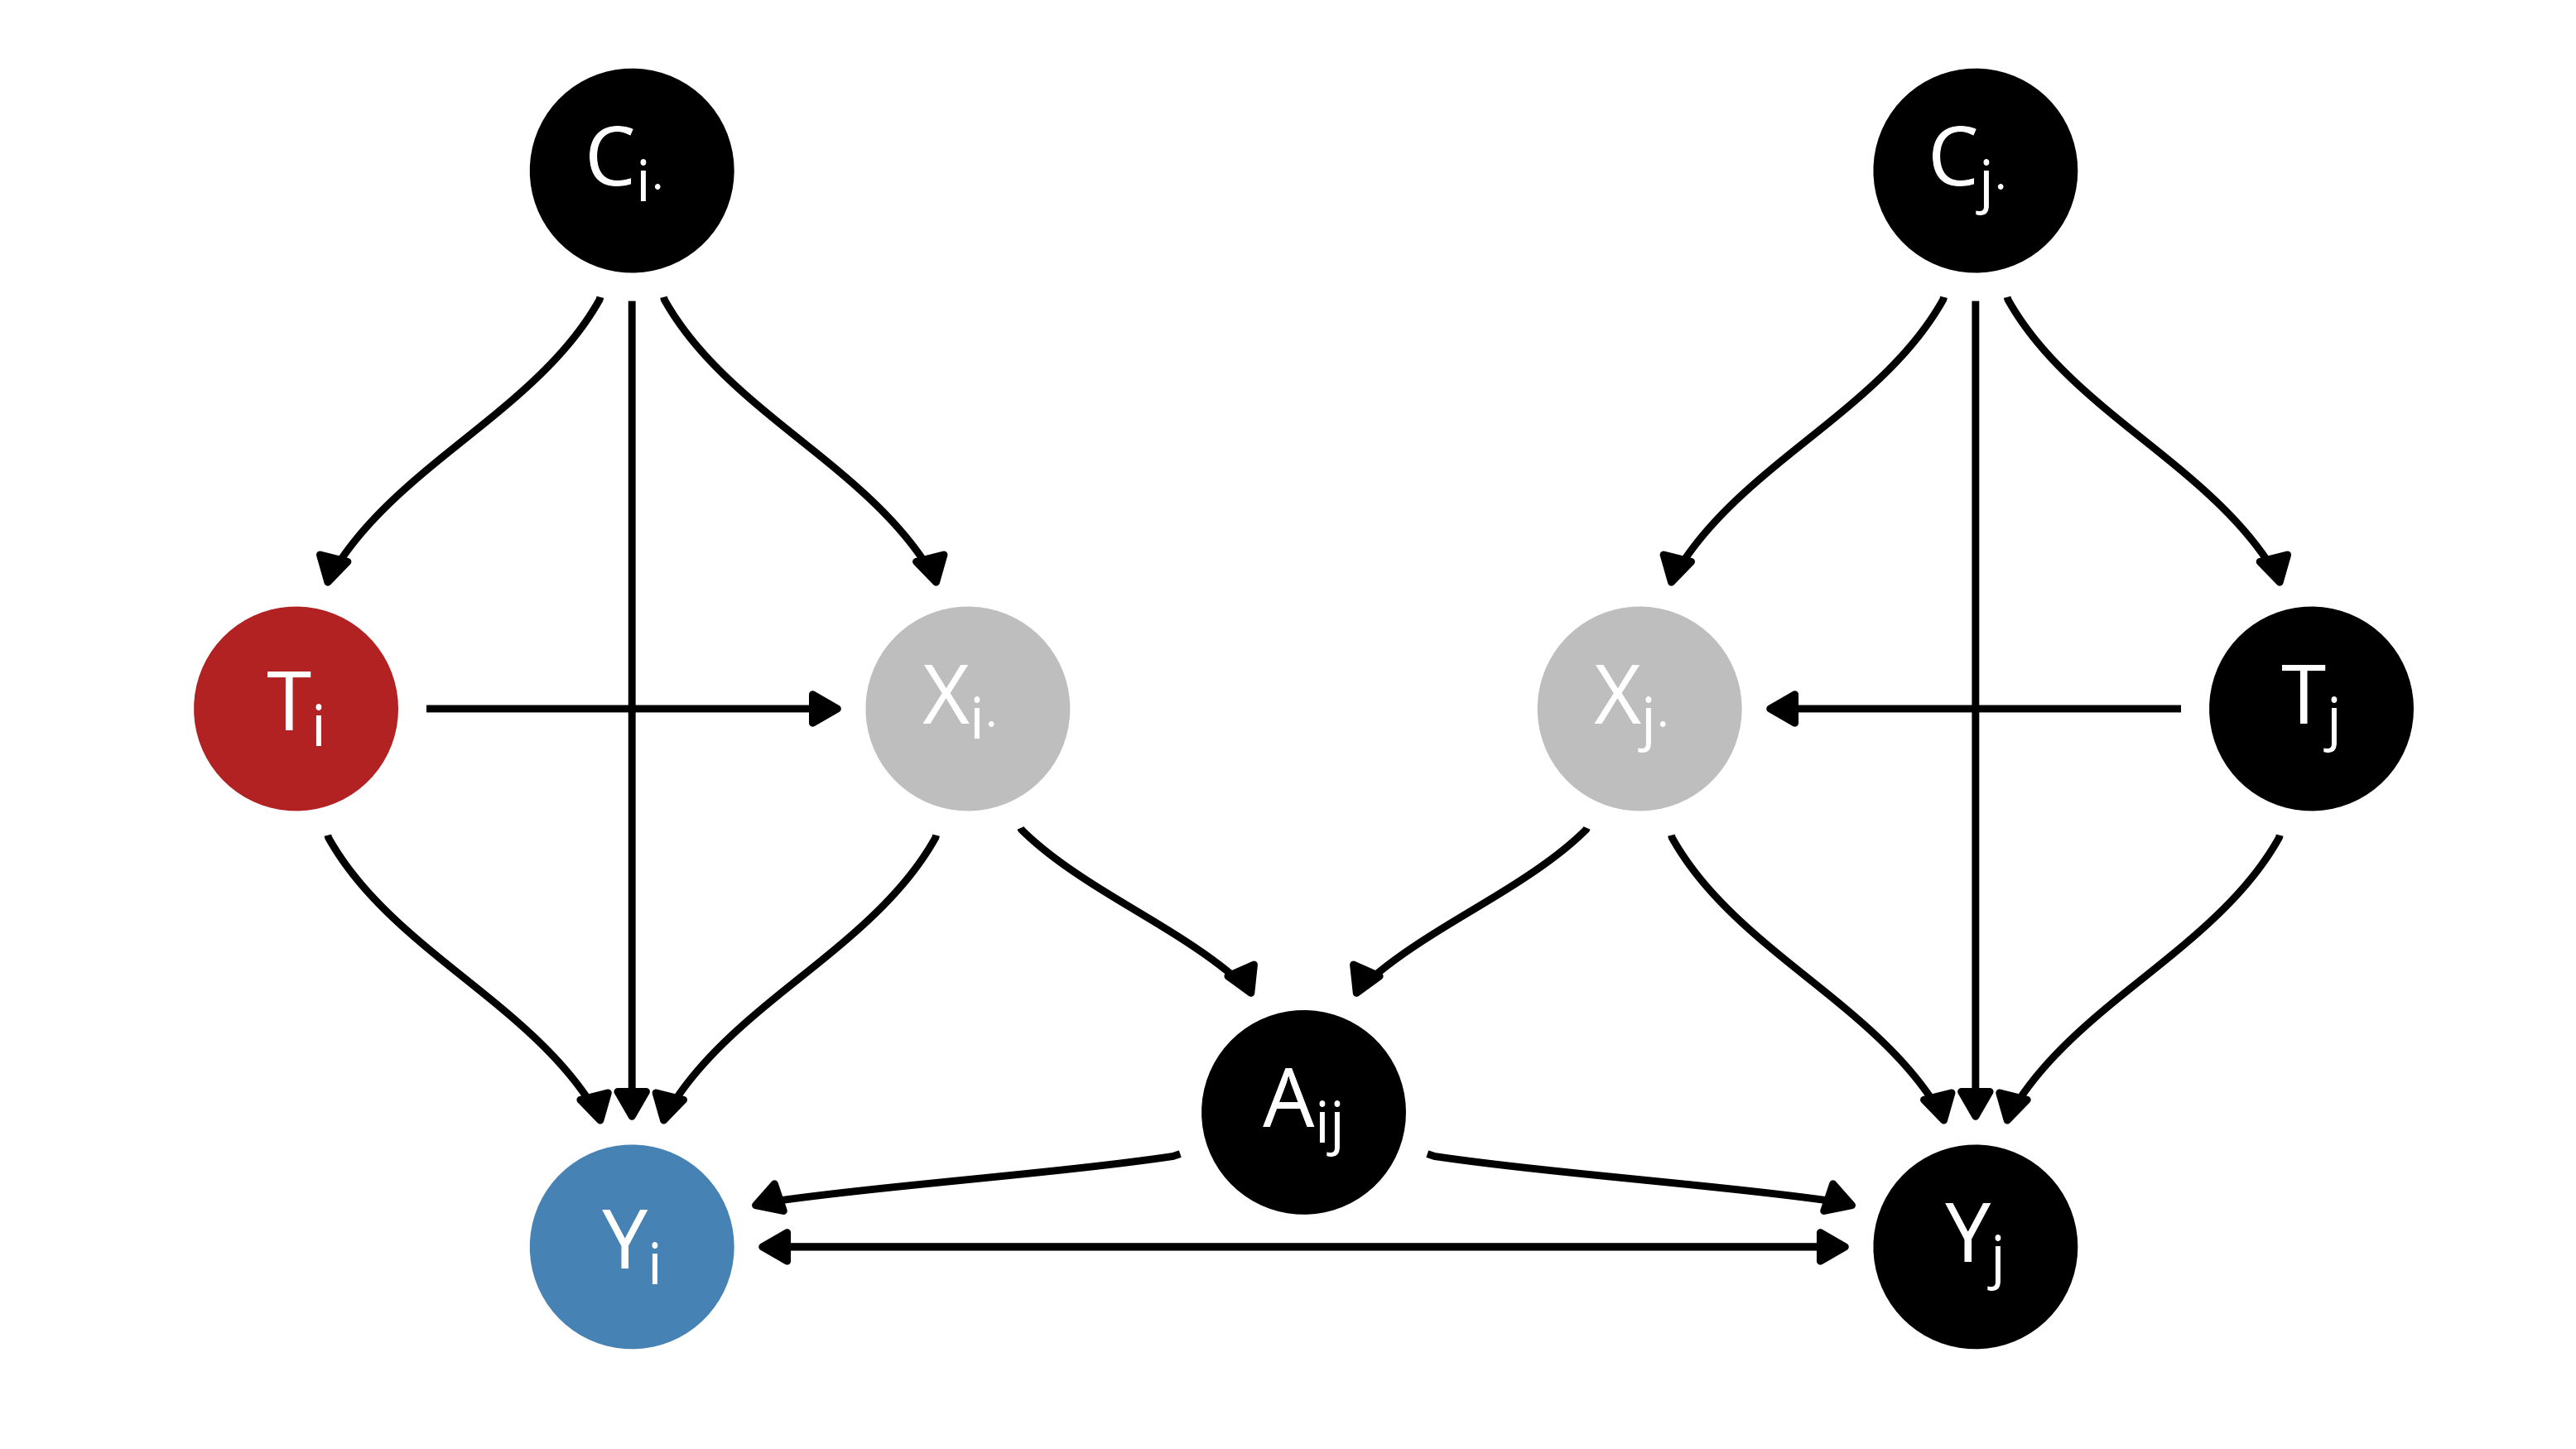
\includegraphics[scale=0.7]{figures/dags/homophily-mediating-contagion-peer.png}
        \label{fig:contagion}
    \end{figure}

\end{frame}

\begin{frame}{Disambiguation: interference ($T_j \to Y_i$) is not allowed}

    \centering

    \begin{figure}
        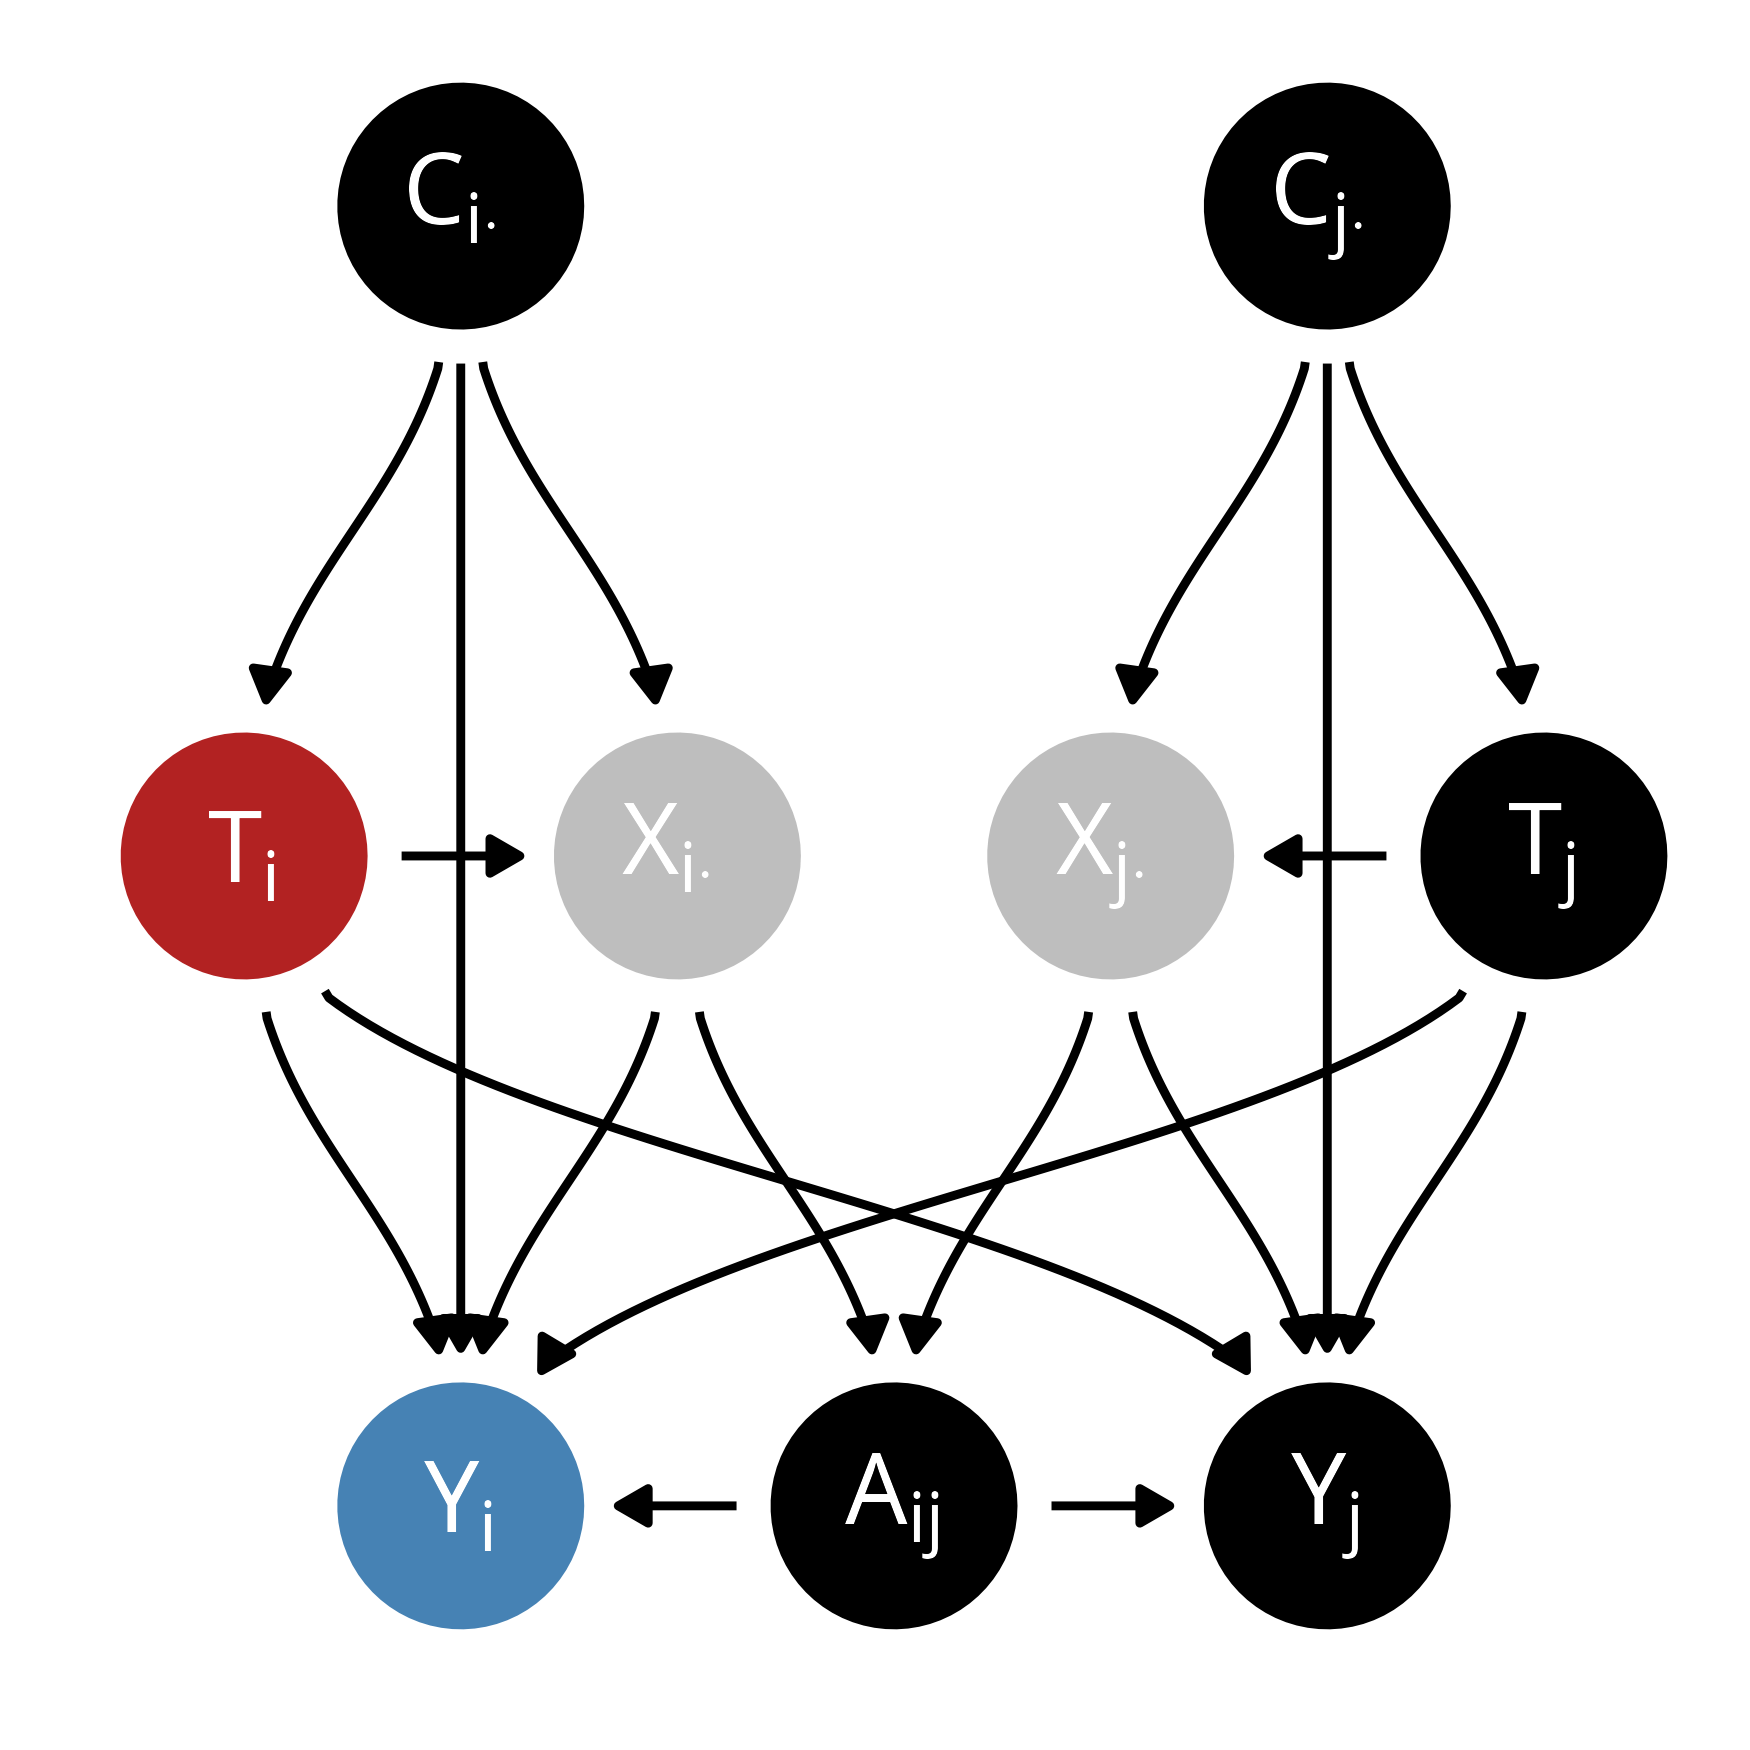
\includegraphics[scale=0.7]{figures/dags/homophily-mediating-interference-peer.png}
        \label{fig:interference}
    \end{figure}

\end{frame}

\begin{frame}{More on interference and contagion}

    Interference and contagion effects are allowed \emph{so long as they happen in the latent space}. Suppose
    \begin{align*}
        \E[\W_{i \cdot}, \X_{i \cdot}]{Y_i}
        = \W_{i \cdot} \betaw + \X_{i \cdot} \beta'_\text{x} + \delta_\text{y} \sum_{j} \X_{i \cdot}^T \X_{j \cdot} Y_j
    \end{align*}
    This latent space contagion model is a special parametric case of the regression outcome model (take $\betax = \beta'_\text{x} + \X^T Y \delta_\text{y}$).

\end{frame}

\begin{frame}{Semi-parametric network model}
    Let $A \in \R^{n \times n}$ be a random symmetric matrix, such as the adjacency matrix of an undirected graph. Let $\Apop = \E[\X]{A} = \X \X^T$ be the expectation of $A$ conditional on $\X \in \R^{n \times d}$, which has independent and identically distributed rows $\X_{1 \cdot}, \dots, \X_{n \cdot}$. That is, $\Apop$ has $\rank \paren*{\Apop} = d$ and is positive semi-definite with eigenvalues $\lambda_1 \ge \lambda_2 \ge \cdots \ge \lambda_d > 0 = \lambda_{d+1} = \cdots = \lambda_n$. Conditional on $\X$, the upper-triangular elements of $A - \Apop$ are independent $(\nu_n, b_n)$-sub-gamma random variables.
\end{frame}


\begin{frame}{Semi-parametric network model: identification of $\X$}

    $\Apop = \X \X^T = (\X Q) (\X Q)^T$ for any $d \times d$ orthogonal matrix $Q$, the latent positions $\X$ are only identifiable up to an orthogonal transformation.
\end{frame}

\begin{frame}{Choosing $\widehat{d}$: do a multiverse analysis}

    \centering

    \begin{figure}
        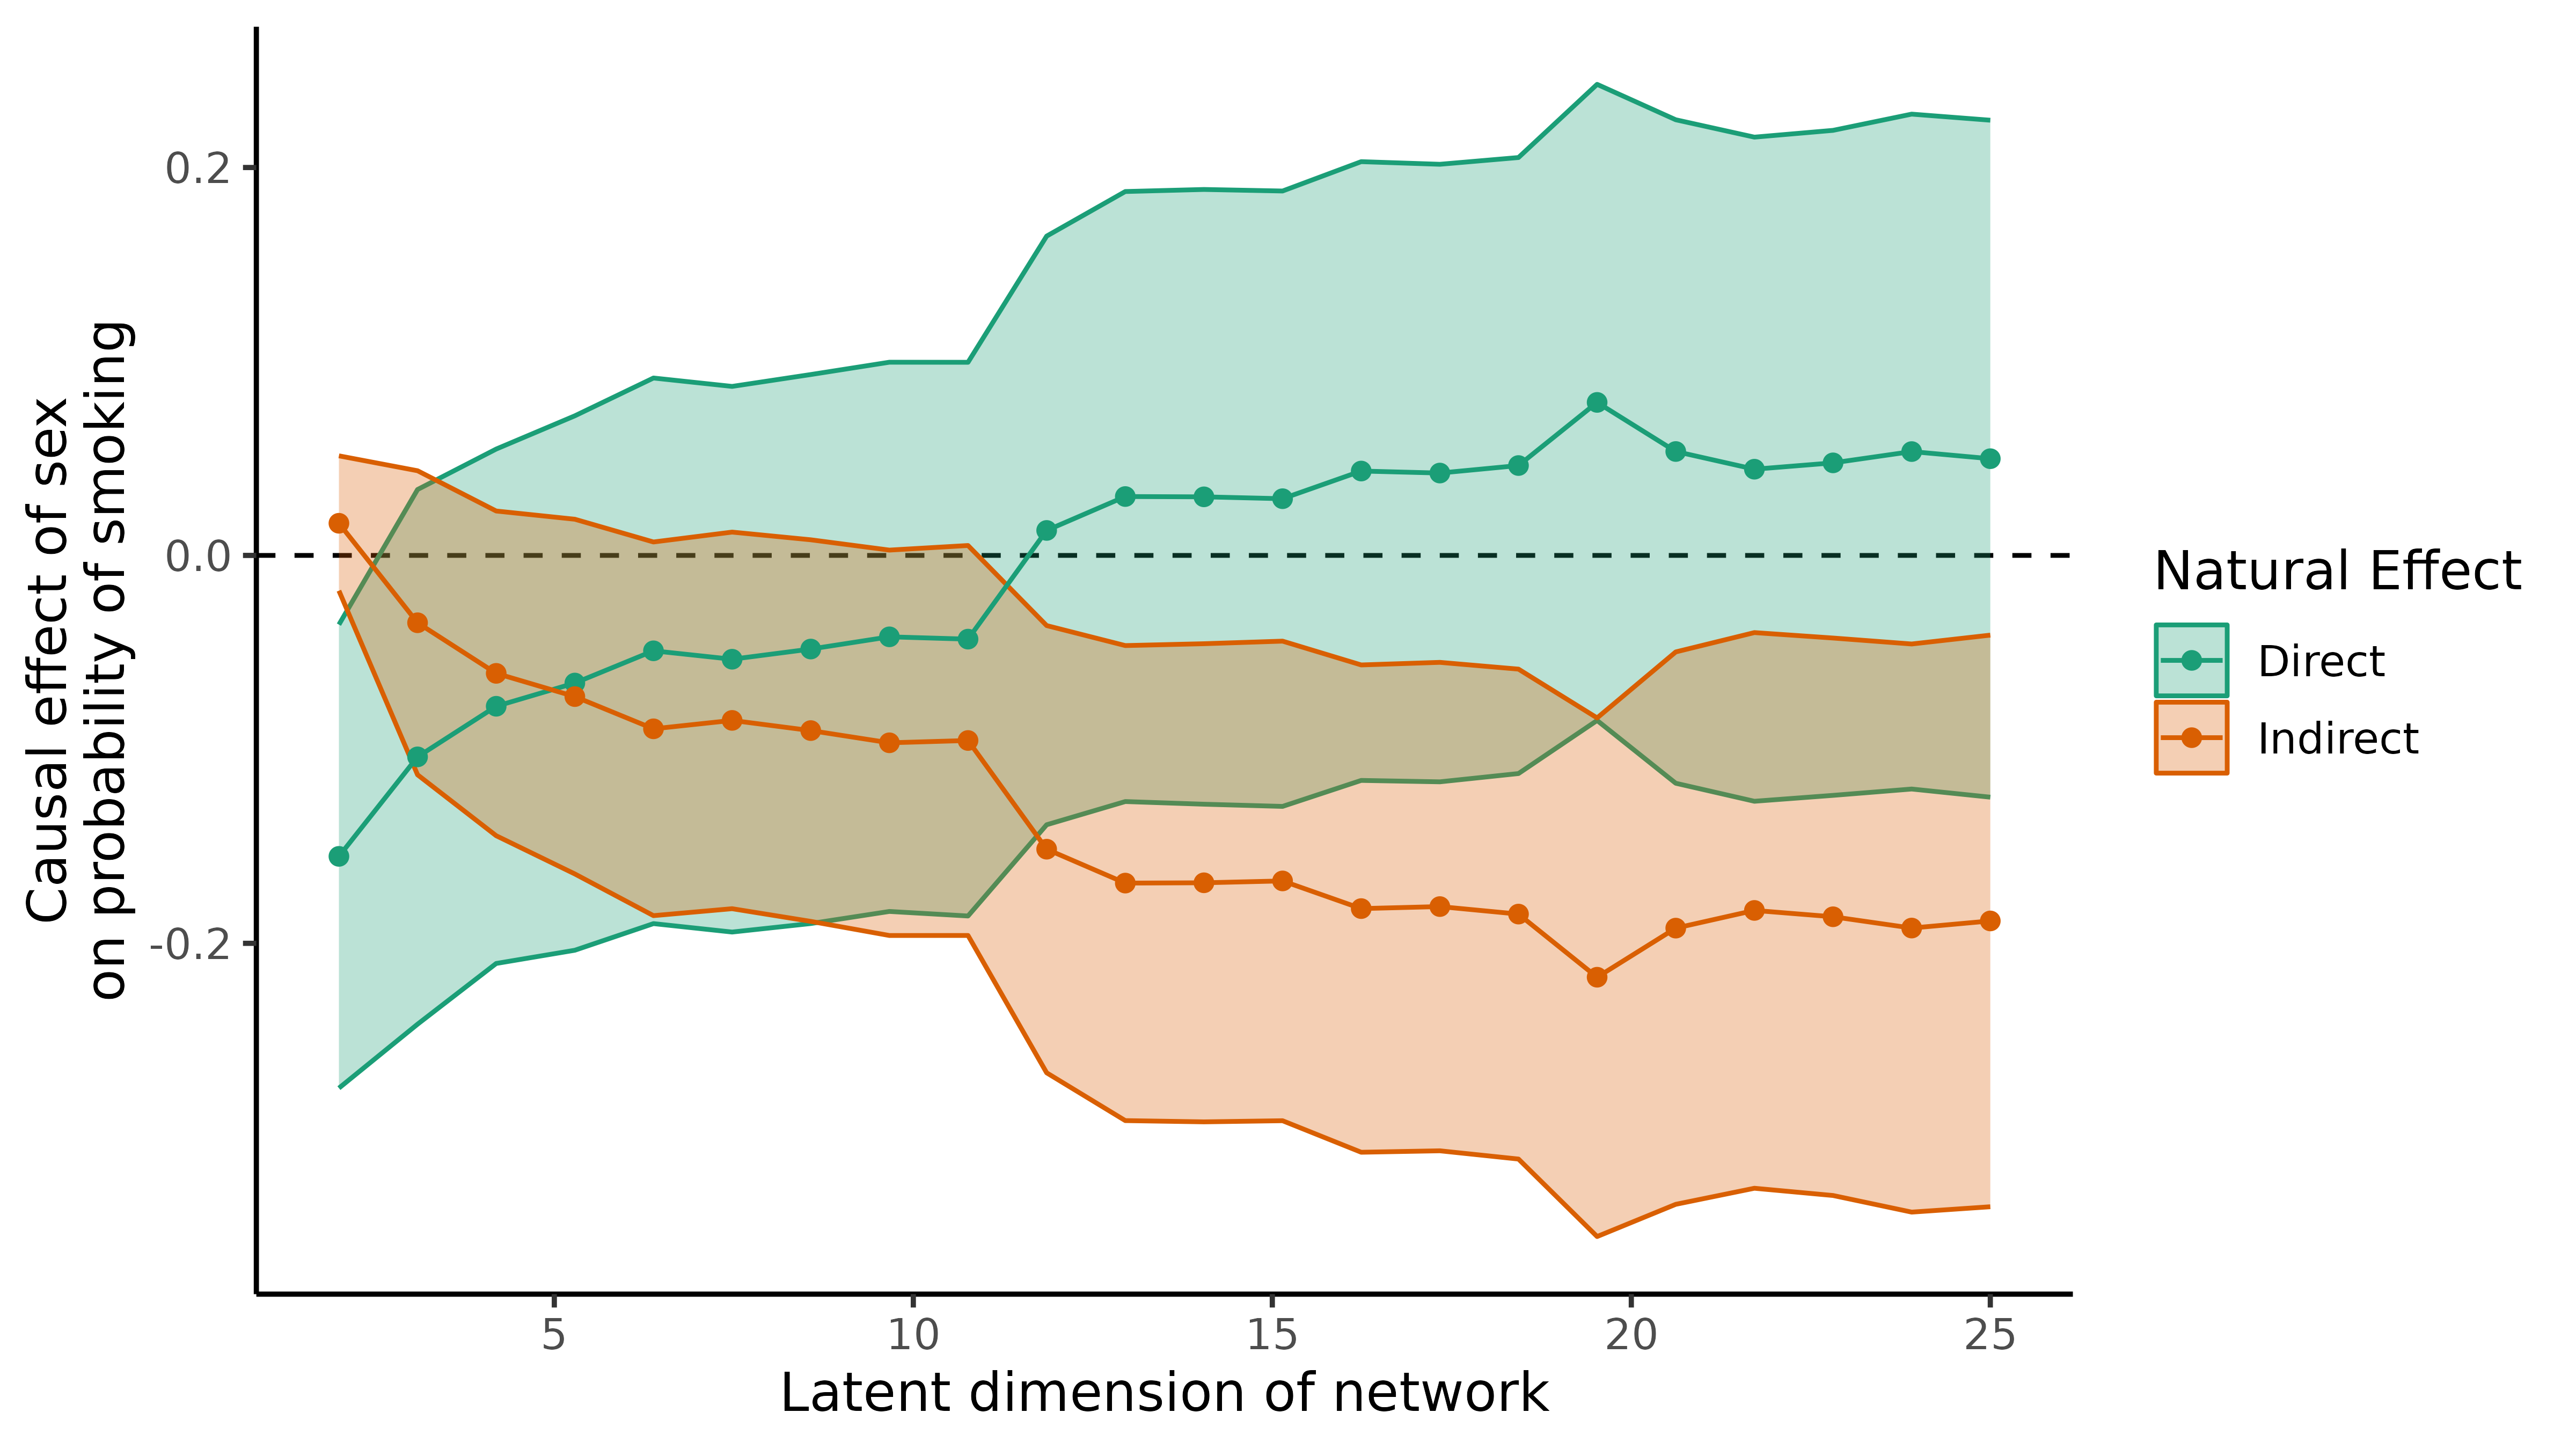
\includegraphics[width=\textwidth]{figures/glasgow-effects.png}
    \end{figure}

\end{frame}

\begin{frame}{Choosing $\widehat{d}$: overestimating the embedding dimension is fine}

    \centering

    \begin{figure}
        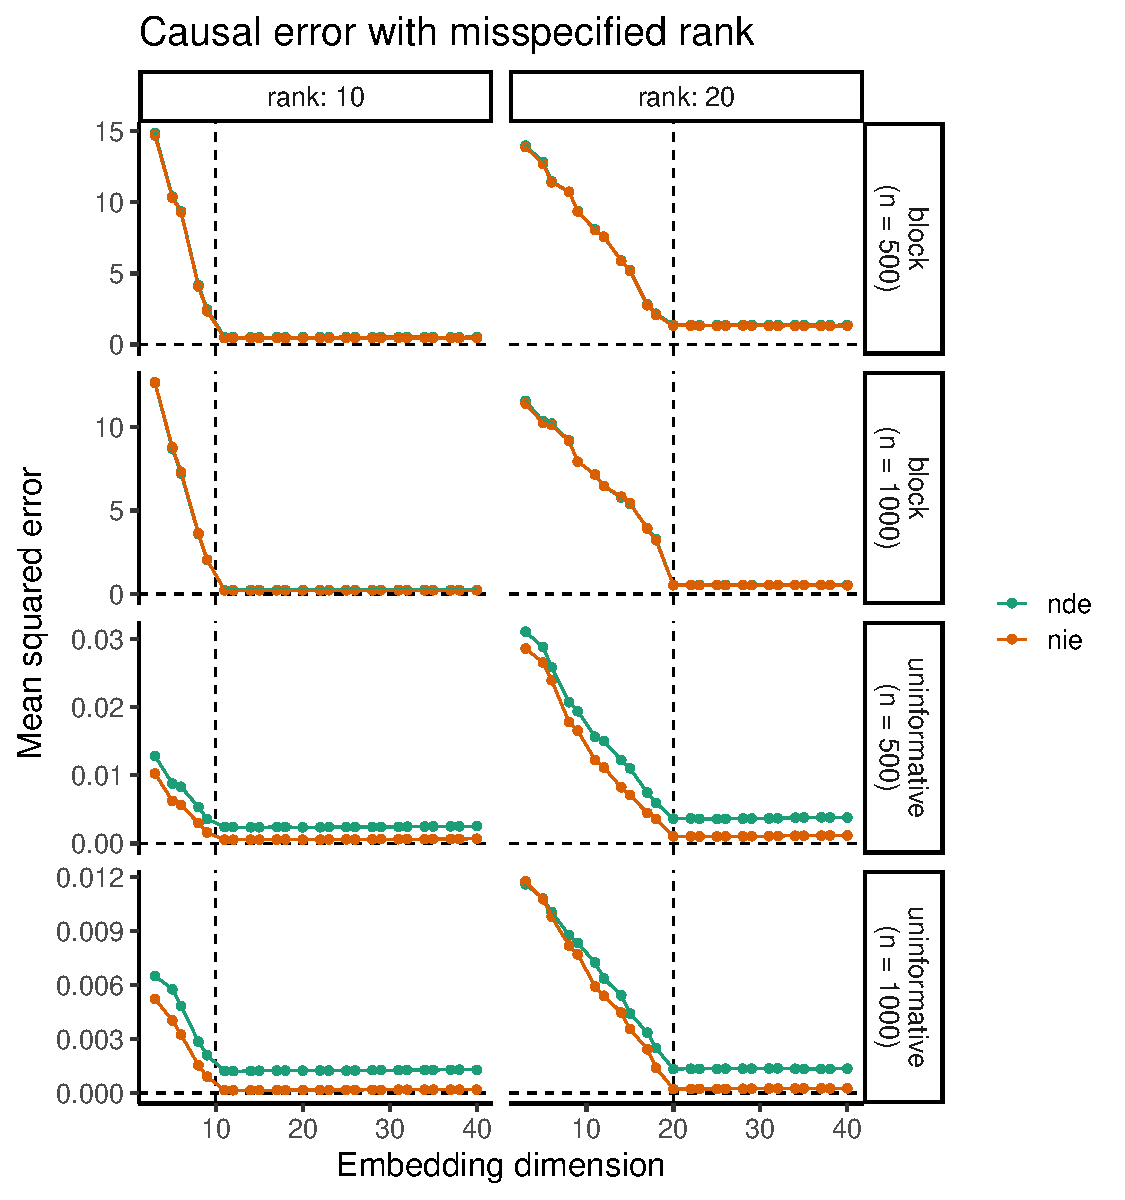
\includegraphics[width=0.7\textwidth]{figures/misspecification/loss_average.pdf}
    \end{figure}

\end{frame}

\begin{frame}{Identifying assumptions}

    The random variables $(Y_i, Y_i(t, x), \X_{i \cdot}, \X_{i \cdot}(t), C_{i \cdot}, T_i)$ are independent over $i \in [n]$ and obey the following three properties.
    \begin{enumerate}
        \item Consistency: \vspace{-3mm}
              \begin{equation*} \begin{aligned}
                       & \text{if $T_i = t$, then $\X_{i \cdot}(t) = \X_{i \cdot}$ with probability 1, and}    \\
                       & \text{if $T_i = t$ and $\X_{i \cdot} = x$, then $Y_i(t, x) = Y_i$ with probability 1}
                      \vspace{-2mm}
                  \end{aligned} \end{equation*}
        \item Sequential ignorability:
              \begin{equation*}
                  \set{Y_i(t^*, x), \X_{i \cdot}(t)} \indep T_i \cond \C_{i \cdot}
                  ~~~\text{ and }~~~
                  \set{Y_i(t^*, x)} \indep \X_{i \cdot}  \cond T_i = t, \C_{i \cdot}
              \end{equation*}
        \item Positivity:
              \begin{equation*}
                  \begin{aligned}
                      \P[T_i, \C_{i \cdot}]{x} & > 0 \text{ for each }  x \in \supp(\X_{i \cdot}) \\
                      \P[\C_{i \cdot}]{t}      & > 0 \text{ for each }  t \in \supp(T_i)
                  \end{aligned}
              \end{equation*}
    \end{enumerate}

\end{frame}

% \begin{frame}{Interventions on a network}

%     \begin{figure}
%         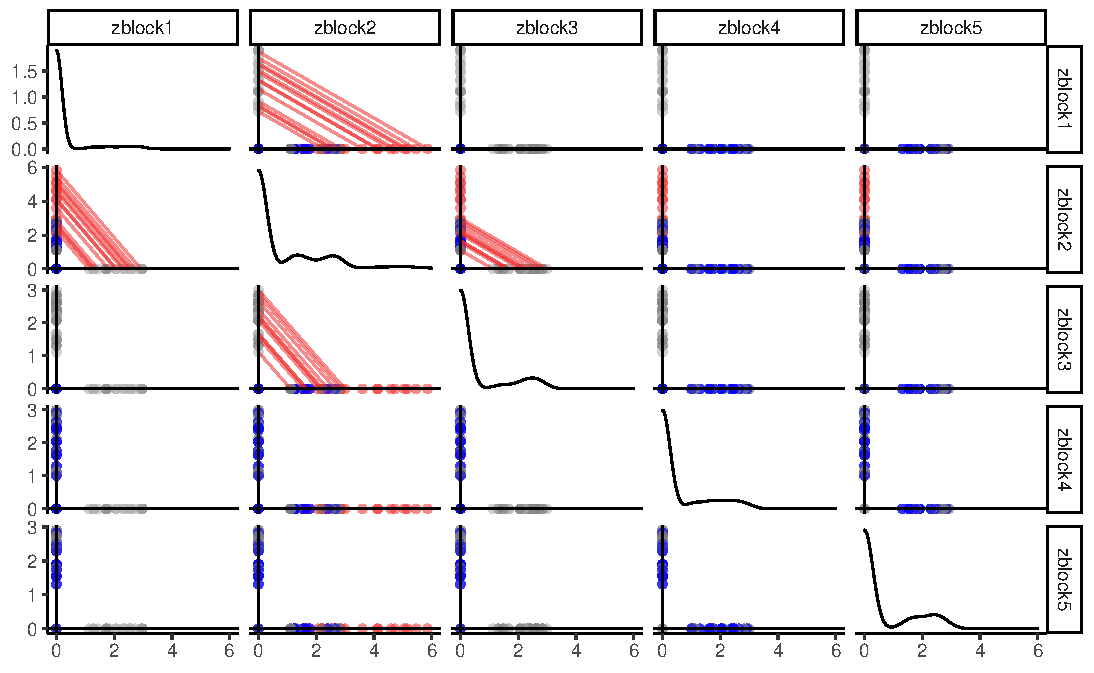
\includegraphics[width=\textwidth]{figures/intervention.pdf}
%         \caption{Canonical intervention when $\C$ is highly informative.}
%         \label{fig:intervention}
%     \end{figure}
% \end{frame}

% \begin{frame}{Interventions on a network}

%     \begin{align*}
%         \underbrace{\E[T_i, \C_{i \cdot}]{\Z_{i \cdot}}}_{\R^{1 \times d}}
%          & = \underbrace{\thetazero}_{\R^{1 \times d}}
%         + \underbrace{T_i}_{\{0, 1\}} \underbrace{\thetat}_{\R^{1 \times d}}
%         + \underbrace{\C_{i \cdot}}_{\R^{1 \times p}} \underbrace{\Thetac}_{\R^{p \times d}}
%         + \underbrace{T_i}_{\{0, 1\}} \underbrace{\C_{i \cdot}}_{\R^{1 \times p}} \underbrace{\Thetatc}_{\R^{p \times d}}.
%     \end{align*}

%     In Figure \ref{fig:intervention}, $\C$ are latent parameters for a DC-SBM and $\thetazero = \vec 0, \thetat = \vec 0, \Thetac = I_k$ and

%     \begin{align*}
%         \Thetatc =
%         \begin{bmatrix}
%             -1 & 2 & 0  & 0 & 0 \\
%             0  & 0 & 0  & 0 & 0 \\
%             0  & 1 & -1 & 0 & 0 \\
%             0  & 0 & 0  & 0 & 0 \\
%             0  & 0 & 0  & 0 & 0 \\
%         \end{bmatrix}
%     \end{align*}
% \end{frame}

\begin{frame}{Interventions allowed}

    Provided that controls $\C_{i \cdot}$ are sufficiently informative about group membership $\X_{i \cdot}$, treatment $T_i$ is allowed to cause:

    \begin{itemize}
        \item Changes in popularity within a group
        \item Movement to a new friend group
        \item Becoming a member of a new friend group while remaining in current friend group
        \item Friendships becoming more or less likely between distinct friend groups
        \item Combinations of the above
    \end{itemize}

    See Appendix of manuscript for details.

\end{frame}

\bibliographystyle{chicago}
\bibliography{references}

\end{document}